\section{Dimer Models}

\begin{frame}{Dimer Models}
    \begin{definition}
        \justifying
        A \textbf{dimer model} is a finite bipartite graph embedded into a compact oriented surface whose nodes and edges form a polygonal cell decomposition of that surface.
    \end{definition}

    \begin{itemize}
        \item Actively studied in theoretical physics: connections to mirror symmetry
        
        \item Interesting source of quivers
    \end{itemize}
\end{frame}

\begin{frame}{Dimer Quiver}
    The \textbf{dimer quiver} of a dimer model is obtained by:
    \begin{itemize}
        \item Taking the dual of the dimer model and
        \item Orienting the faces of the dual clockwise about white vertices and counterclockwise about black vertices
    \end{itemize}
    \begin{center}
        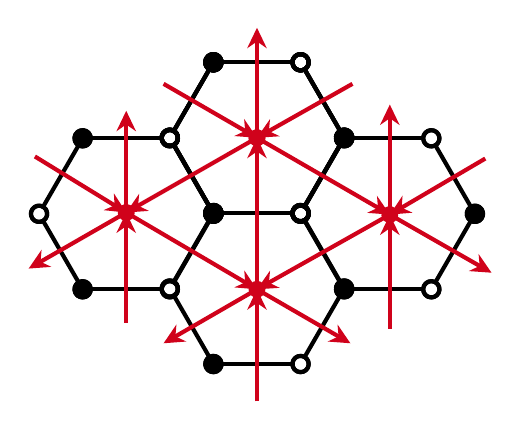
\begin{tikzpicture}[x=0.75pt,y=0.75pt,yscale=-1,xscale=1]
            %uncomment if require: \path (0,410); %set diagram left start at 0, and has height of 410
            
            %Straight Lines [id:da4784732403080071] 
            \draw [line width=1.5]    (249.46,131.47) -- (269,97.63) ;
            \draw [shift={(269,97.63)}, rotate = 300] [color={rgb, 255:red, 0; green, 0; blue, 0 }  ][fill={rgb, 255:red, 0; green, 0; blue, 0 }  ][line width=1.5]      (0, 0) circle [x radius= 3.92, y radius= 3.92]   ;
            \draw [shift={(248,134)}, rotate = 300] [color={rgb, 255:red, 0; green, 0; blue, 0 }  ][line width=1.5]      (0, 0) circle [x radius= 3.92, y radius= 3.92]   ;
            %Straight Lines [id:da5469273551671134] 
            \draw [line width=1.5]    (308.08,97.63) -- (269,97.63) ;
            \draw [shift={(269,97.63)}, rotate = 180] [color={rgb, 255:red, 0; green, 0; blue, 0 }  ][fill={rgb, 255:red, 0; green, 0; blue, 0 }  ][line width=1.5]      (0, 0) circle [x radius= 3.92, y radius= 3.92]   ;
            \draw [shift={(311,97.63)}, rotate = 180] [color={rgb, 255:red, 0; green, 0; blue, 0 }  ][line width=1.5]      (0, 0) circle [x radius= 3.92, y radius= 3.92]   ;
            %Straight Lines [id:da4973607875390542] 
            \draw [line width=1.5]    (312.46,100.16) -- (332,134) ;
            \draw [shift={(332,134)}, rotate = 60] [color={rgb, 255:red, 0; green, 0; blue, 0 }  ][fill={rgb, 255:red, 0; green, 0; blue, 0 }  ][line width=1.5]      (0, 0) circle [x radius= 3.92, y radius= 3.92]   ;
            \draw [shift={(311,97.63)}, rotate = 60] [color={rgb, 255:red, 0; green, 0; blue, 0 }  ][line width=1.5]      (0, 0) circle [x radius= 3.92, y radius= 3.92]   ;
            %Straight Lines [id:da7735402625393233] 
            \draw [line width=1.5]    (312.46,167.84) -- (332,134) ;
            \draw [shift={(332,134)}, rotate = 300] [color={rgb, 255:red, 0; green, 0; blue, 0 }  ][fill={rgb, 255:red, 0; green, 0; blue, 0 }  ][line width=1.5]      (0, 0) circle [x radius= 3.92, y radius= 3.92]   ;
            \draw [shift={(311,170.37)}, rotate = 300] [color={rgb, 255:red, 0; green, 0; blue, 0 }  ][line width=1.5]      (0, 0) circle [x radius= 3.92, y radius= 3.92]   ;
            %Straight Lines [id:da10900558892598333] 
            \draw [line width=1.5]    (308.08,170.37) -- (269,170.37) ;
            \draw [shift={(269,170.37)}, rotate = 180] [color={rgb, 255:red, 0; green, 0; blue, 0 }  ][fill={rgb, 255:red, 0; green, 0; blue, 0 }  ][line width=1.5]      (0, 0) circle [x radius= 3.92, y radius= 3.92]   ;
            \draw [shift={(311,170.37)}, rotate = 180] [color={rgb, 255:red, 0; green, 0; blue, 0 }  ][line width=1.5]      (0, 0) circle [x radius= 3.92, y radius= 3.92]   ;
            %Straight Lines [id:da36966648789613377] 
            \draw [line width=1.5]    (249.46,136.53) -- (269,170.37) ;
            \draw [shift={(269,170.37)}, rotate = 60] [color={rgb, 255:red, 0; green, 0; blue, 0 }  ][fill={rgb, 255:red, 0; green, 0; blue, 0 }  ][line width=1.5]      (0, 0) circle [x radius= 3.92, y radius= 3.92]   ;
            \draw [shift={(248,134)}, rotate = 60] [color={rgb, 255:red, 0; green, 0; blue, 0 }  ][line width=1.5]      (0, 0) circle [x radius= 3.92, y radius= 3.92]   ;
            %Straight Lines [id:da3119443766311246] 
            \draw [line width=1.5]    (249.46,131.47) -- (269,97.63) ;
            \draw [shift={(269,97.63)}, rotate = 300] [color={rgb, 255:red, 0; green, 0; blue, 0 }  ][fill={rgb, 255:red, 0; green, 0; blue, 0 }  ][line width=1.5]      (0, 0) circle [x radius= 3.92, y radius= 3.92]   ;
            \draw [shift={(248,134)}, rotate = 300] [color={rgb, 255:red, 0; green, 0; blue, 0 }  ][line width=1.5]      (0, 0) circle [x radius= 3.92, y radius= 3.92]   ;
            %Straight Lines [id:da027848228347852277] 
            \draw [line width=1.5]    (308.08,97.63) -- (269,97.63) ;
            \draw [shift={(269,97.63)}, rotate = 180] [color={rgb, 255:red, 0; green, 0; blue, 0 }  ][fill={rgb, 255:red, 0; green, 0; blue, 0 }  ][line width=1.5]      (0, 0) circle [x radius= 3.92, y radius= 3.92]   ;
            \draw [shift={(311,97.63)}, rotate = 180] [color={rgb, 255:red, 0; green, 0; blue, 0 }  ][line width=1.5]      (0, 0) circle [x radius= 3.92, y radius= 3.92]   ;
            %Straight Lines [id:da618096670806669] 
            \draw [line width=1.5]    (312.46,100.16) -- (332,134) ;
            \draw [shift={(332,134)}, rotate = 60] [color={rgb, 255:red, 0; green, 0; blue, 0 }  ][fill={rgb, 255:red, 0; green, 0; blue, 0 }  ][line width=1.5]      (0, 0) circle [x radius= 3.92, y radius= 3.92]   ;
            \draw [shift={(311,97.63)}, rotate = 60] [color={rgb, 255:red, 0; green, 0; blue, 0 }  ][line width=1.5]      (0, 0) circle [x radius= 3.92, y radius= 3.92]   ;
            %Straight Lines [id:da7251340314451928] 
            \draw [line width=1.5]    (312.46,167.84) -- (332,134) ;
            \draw [shift={(332,134)}, rotate = 300] [color={rgb, 255:red, 0; green, 0; blue, 0 }  ][fill={rgb, 255:red, 0; green, 0; blue, 0 }  ][line width=1.5]      (0, 0) circle [x radius= 3.92, y radius= 3.92]   ;
            \draw [shift={(311,170.37)}, rotate = 300] [color={rgb, 255:red, 0; green, 0; blue, 0 }  ][line width=1.5]      (0, 0) circle [x radius= 3.92, y radius= 3.92]   ;
            %Straight Lines [id:da8025907125285042] 
            \draw [line width=1.5]    (308.08,170.37) -- (269,170.37) ;
            \draw [shift={(269,170.37)}, rotate = 180] [color={rgb, 255:red, 0; green, 0; blue, 0 }  ][fill={rgb, 255:red, 0; green, 0; blue, 0 }  ][line width=1.5]      (0, 0) circle [x radius= 3.92, y radius= 3.92]   ;
            \draw [shift={(311,170.37)}, rotate = 180] [color={rgb, 255:red, 0; green, 0; blue, 0 }  ][line width=1.5]      (0, 0) circle [x radius= 3.92, y radius= 3.92]   ;
            %Straight Lines [id:da9676076737667815] 
            \draw [line width=1.5]    (249.46,136.53) -- (269,170.37) ;
            \draw [shift={(269,170.37)}, rotate = 60] [color={rgb, 255:red, 0; green, 0; blue, 0 }  ][fill={rgb, 255:red, 0; green, 0; blue, 0 }  ][line width=1.5]      (0, 0) circle [x radius= 3.92, y radius= 3.92]   ;
            \draw [shift={(248,134)}, rotate = 60] [color={rgb, 255:red, 0; green, 0; blue, 0 }  ][line width=1.5]      (0, 0) circle [x radius= 3.92, y radius= 3.92]   ;
            %Straight Lines [id:da5504214107467595] 
            \draw [line width=1.5]    (249.46,131.47) -- (269,97.63) ;
            \draw [shift={(269,97.63)}, rotate = 300] [color={rgb, 255:red, 0; green, 0; blue, 0 }  ][fill={rgb, 255:red, 0; green, 0; blue, 0 }  ][line width=1.5]      (0, 0) circle [x radius= 3.92, y radius= 3.92]   ;
            \draw [shift={(248,134)}, rotate = 300] [color={rgb, 255:red, 0; green, 0; blue, 0 }  ][line width=1.5]      (0, 0) circle [x radius= 3.92, y radius= 3.92]   ;
            %Straight Lines [id:da8614354758228218] 
            \draw [line width=1.5]    (308.08,97.63) -- (269,97.63) ;
            \draw [shift={(269,97.63)}, rotate = 180] [color={rgb, 255:red, 0; green, 0; blue, 0 }  ][fill={rgb, 255:red, 0; green, 0; blue, 0 }  ][line width=1.5]      (0, 0) circle [x radius= 3.92, y radius= 3.92]   ;
            \draw [shift={(311,97.63)}, rotate = 180] [color={rgb, 255:red, 0; green, 0; blue, 0 }  ][line width=1.5]      (0, 0) circle [x radius= 3.92, y radius= 3.92]   ;
            %Straight Lines [id:da6150615607355029] 
            \draw [line width=1.5]    (312.46,100.16) -- (332,134) ;
            \draw [shift={(332,134)}, rotate = 60] [color={rgb, 255:red, 0; green, 0; blue, 0 }  ][fill={rgb, 255:red, 0; green, 0; blue, 0 }  ][line width=1.5]      (0, 0) circle [x radius= 3.92, y radius= 3.92]   ;
            \draw [shift={(311,97.63)}, rotate = 60] [color={rgb, 255:red, 0; green, 0; blue, 0 }  ][line width=1.5]      (0, 0) circle [x radius= 3.92, y radius= 3.92]   ;
            %Straight Lines [id:da25023270439015777] 
            \draw [line width=1.5]    (312.46,167.84) -- (332,134) ;
            \draw [shift={(332,134)}, rotate = 300] [color={rgb, 255:red, 0; green, 0; blue, 0 }  ][fill={rgb, 255:red, 0; green, 0; blue, 0 }  ][line width=1.5]      (0, 0) circle [x radius= 3.92, y radius= 3.92]   ;
            \draw [shift={(311,170.37)}, rotate = 300] [color={rgb, 255:red, 0; green, 0; blue, 0 }  ][line width=1.5]      (0, 0) circle [x radius= 3.92, y radius= 3.92]   ;
            %Straight Lines [id:da8047101799810017] 
            \draw [line width=1.5]    (308.08,170.37) -- (269,170.37) ;
            \draw [shift={(269,170.37)}, rotate = 180] [color={rgb, 255:red, 0; green, 0; blue, 0 }  ][fill={rgb, 255:red, 0; green, 0; blue, 0 }  ][line width=1.5]      (0, 0) circle [x radius= 3.92, y radius= 3.92]   ;
            \draw [shift={(311,170.37)}, rotate = 180] [color={rgb, 255:red, 0; green, 0; blue, 0 }  ][line width=1.5]      (0, 0) circle [x radius= 3.92, y radius= 3.92]   ;
            %Straight Lines [id:da35431168164006865] 
            \draw [line width=1.5]    (249.46,136.53) -- (269,170.37) ;
            \draw [shift={(269,170.37)}, rotate = 60] [color={rgb, 255:red, 0; green, 0; blue, 0 }  ][fill={rgb, 255:red, 0; green, 0; blue, 0 }  ][line width=1.5]      (0, 0) circle [x radius= 3.92, y radius= 3.92]   ;
            \draw [shift={(248,134)}, rotate = 60] [color={rgb, 255:red, 0; green, 0; blue, 0 }  ][line width=1.5]      (0, 0) circle [x radius= 3.92, y radius= 3.92]   ;
            %Straight Lines [id:da5418595626998984] 
            \draw [line width=1.5]    (312.46,168.1) -- (332,134.25) ;
            \draw [shift={(332,134.25)}, rotate = 300] [color={rgb, 255:red, 0; green, 0; blue, 0 }  ][fill={rgb, 255:red, 0; green, 0; blue, 0 }  ][line width=1.5]      (0, 0) circle [x radius= 3.92, y radius= 3.92]   ;
            \draw [shift={(311,170.63)}, rotate = 300] [color={rgb, 255:red, 0; green, 0; blue, 0 }  ][line width=1.5]      (0, 0) circle [x radius= 3.92, y radius= 3.92]   ;
            %Straight Lines [id:da583251097437717] 
            \draw [line width=1.5]    (371.08,134.25) -- (332,134.25) ;
            \draw [shift={(332,134.25)}, rotate = 180] [color={rgb, 255:red, 0; green, 0; blue, 0 }  ][fill={rgb, 255:red, 0; green, 0; blue, 0 }  ][line width=1.5]      (0, 0) circle [x radius= 3.92, y radius= 3.92]   ;
            \draw [shift={(374,134.25)}, rotate = 180] [color={rgb, 255:red, 0; green, 0; blue, 0 }  ][line width=1.5]      (0, 0) circle [x radius= 3.92, y radius= 3.92]   ;
            %Straight Lines [id:da6400555719185436] 
            \draw [line width=1.5]    (375.46,136.78) -- (395,170.63) ;
            \draw [shift={(395,170.63)}, rotate = 60] [color={rgb, 255:red, 0; green, 0; blue, 0 }  ][fill={rgb, 255:red, 0; green, 0; blue, 0 }  ][line width=1.5]      (0, 0) circle [x radius= 3.92, y radius= 3.92]   ;
            \draw [shift={(374,134.25)}, rotate = 60] [color={rgb, 255:red, 0; green, 0; blue, 0 }  ][line width=1.5]      (0, 0) circle [x radius= 3.92, y radius= 3.92]   ;
            %Straight Lines [id:da44447926401156046] 
            \draw [line width=1.5]    (375.46,204.47) -- (395,170.63) ;
            \draw [shift={(395,170.63)}, rotate = 300] [color={rgb, 255:red, 0; green, 0; blue, 0 }  ][fill={rgb, 255:red, 0; green, 0; blue, 0 }  ][line width=1.5]      (0, 0) circle [x radius= 3.92, y radius= 3.92]   ;
            \draw [shift={(374,207)}, rotate = 300] [color={rgb, 255:red, 0; green, 0; blue, 0 }  ][line width=1.5]      (0, 0) circle [x radius= 3.92, y radius= 3.92]   ;
            %Straight Lines [id:da1314711869995] 
            \draw [line width=1.5]    (371.08,207) -- (332,207) ;
            \draw [shift={(332,207)}, rotate = 180] [color={rgb, 255:red, 0; green, 0; blue, 0 }  ][fill={rgb, 255:red, 0; green, 0; blue, 0 }  ][line width=1.5]      (0, 0) circle [x radius= 3.92, y radius= 3.92]   ;
            \draw [shift={(374,207)}, rotate = 180] [color={rgb, 255:red, 0; green, 0; blue, 0 }  ][line width=1.5]      (0, 0) circle [x radius= 3.92, y radius= 3.92]   ;
            %Straight Lines [id:da6241072496776653] 
            \draw [line width=1.5]    (312.46,173.16) -- (332,207) ;
            \draw [shift={(332,207)}, rotate = 60] [color={rgb, 255:red, 0; green, 0; blue, 0 }  ][fill={rgb, 255:red, 0; green, 0; blue, 0 }  ][line width=1.5]      (0, 0) circle [x radius= 3.92, y radius= 3.92]   ;
            \draw [shift={(311,170.63)}, rotate = 60] [color={rgb, 255:red, 0; green, 0; blue, 0 }  ][line width=1.5]      (0, 0) circle [x radius= 3.92, y radius= 3.92]   ;
            %Straight Lines [id:da16265355757683542] 
            \draw [line width=1.5]    (249.46,204.1) -- (269,170.25) ;
            \draw [shift={(269,170.25)}, rotate = 300] [color={rgb, 255:red, 0; green, 0; blue, 0 }  ][fill={rgb, 255:red, 0; green, 0; blue, 0 }  ][line width=1.5]      (0, 0) circle [x radius= 3.92, y radius= 3.92]   ;
            \draw [shift={(248,206.63)}, rotate = 300] [color={rgb, 255:red, 0; green, 0; blue, 0 }  ][line width=1.5]      (0, 0) circle [x radius= 3.92, y radius= 3.92]   ;
            %Straight Lines [id:da7953189925020766] 
            \draw [line width=1.5]    (308.08,170.25) -- (269,170.25) ;
            \draw [shift={(269,170.25)}, rotate = 180] [color={rgb, 255:red, 0; green, 0; blue, 0 }  ][fill={rgb, 255:red, 0; green, 0; blue, 0 }  ][line width=1.5]      (0, 0) circle [x radius= 3.92, y radius= 3.92]   ;
            \draw [shift={(311,170.25)}, rotate = 180] [color={rgb, 255:red, 0; green, 0; blue, 0 }  ][line width=1.5]      (0, 0) circle [x radius= 3.92, y radius= 3.92]   ;
            %Straight Lines [id:da8170083034534992] 
            \draw [line width=1.5]    (312.46,172.78) -- (332,206.63) ;
            \draw [shift={(332,206.63)}, rotate = 60] [color={rgb, 255:red, 0; green, 0; blue, 0 }  ][fill={rgb, 255:red, 0; green, 0; blue, 0 }  ][line width=1.5]      (0, 0) circle [x radius= 3.92, y radius= 3.92]   ;
            \draw [shift={(311,170.25)}, rotate = 60] [color={rgb, 255:red, 0; green, 0; blue, 0 }  ][line width=1.5]      (0, 0) circle [x radius= 3.92, y radius= 3.92]   ;
            %Straight Lines [id:da25041568622714294] 
            \draw [line width=1.5]    (312.46,240.47) -- (332,206.63) ;
            \draw [shift={(332,206.63)}, rotate = 300] [color={rgb, 255:red, 0; green, 0; blue, 0 }  ][fill={rgb, 255:red, 0; green, 0; blue, 0 }  ][line width=1.5]      (0, 0) circle [x radius= 3.92, y radius= 3.92]   ;
            \draw [shift={(311,243)}, rotate = 300] [color={rgb, 255:red, 0; green, 0; blue, 0 }  ][line width=1.5]      (0, 0) circle [x radius= 3.92, y radius= 3.92]   ;
            %Straight Lines [id:da5494944295555454] 
            \draw [line width=1.5]    (308.08,243) -- (269,243) ;
            \draw [shift={(269,243)}, rotate = 180] [color={rgb, 255:red, 0; green, 0; blue, 0 }  ][fill={rgb, 255:red, 0; green, 0; blue, 0 }  ][line width=1.5]      (0, 0) circle [x radius= 3.92, y radius= 3.92]   ;
            \draw [shift={(311,243)}, rotate = 180] [color={rgb, 255:red, 0; green, 0; blue, 0 }  ][line width=1.5]      (0, 0) circle [x radius= 3.92, y radius= 3.92]   ;
            %Straight Lines [id:da39546058883770574] 
            \draw [line width=1.5]    (249.46,209.16) -- (269,243) ;
            \draw [shift={(269,243)}, rotate = 60] [color={rgb, 255:red, 0; green, 0; blue, 0 }  ][fill={rgb, 255:red, 0; green, 0; blue, 0 }  ][line width=1.5]      (0, 0) circle [x radius= 3.92, y radius= 3.92]   ;
            \draw [shift={(248,206.63)}, rotate = 60] [color={rgb, 255:red, 0; green, 0; blue, 0 }  ][line width=1.5]      (0, 0) circle [x radius= 3.92, y radius= 3.92]   ;
            %Straight Lines [id:da3727762671681867] 
            \draw [line width=1.5]    (186.46,168.1) -- (206,134.25) ;
            \draw [shift={(206,134.25)}, rotate = 300] [color={rgb, 255:red, 0; green, 0; blue, 0 }  ][fill={rgb, 255:red, 0; green, 0; blue, 0 }  ][line width=1.5]      (0, 0) circle [x radius= 3.92, y radius= 3.92]   ;
            \draw [shift={(185,170.63)}, rotate = 300] [color={rgb, 255:red, 0; green, 0; blue, 0 }  ][line width=1.5]      (0, 0) circle [x radius= 3.92, y radius= 3.92]   ;
            %Straight Lines [id:da15366725504674705] 
            \draw [line width=1.5]    (245.08,134.25) -- (206,134.25) ;
            \draw [shift={(206,134.25)}, rotate = 180] [color={rgb, 255:red, 0; green, 0; blue, 0 }  ][fill={rgb, 255:red, 0; green, 0; blue, 0 }  ][line width=1.5]      (0, 0) circle [x radius= 3.92, y radius= 3.92]   ;
            \draw [shift={(248,134.25)}, rotate = 180] [color={rgb, 255:red, 0; green, 0; blue, 0 }  ][line width=1.5]      (0, 0) circle [x radius= 3.92, y radius= 3.92]   ;
            %Straight Lines [id:da9843176382072218] 
            \draw [line width=1.5]    (249.46,136.78) -- (269,170.63) ;
            \draw [shift={(269,170.63)}, rotate = 60] [color={rgb, 255:red, 0; green, 0; blue, 0 }  ][fill={rgb, 255:red, 0; green, 0; blue, 0 }  ][line width=1.5]      (0, 0) circle [x radius= 3.92, y radius= 3.92]   ;
            \draw [shift={(248,134.25)}, rotate = 60] [color={rgb, 255:red, 0; green, 0; blue, 0 }  ][line width=1.5]      (0, 0) circle [x radius= 3.92, y radius= 3.92]   ;
            %Straight Lines [id:da463792797830324] 
            \draw [line width=1.5]    (249.46,204.47) -- (269,170.63) ;
            \draw [shift={(269,170.63)}, rotate = 300] [color={rgb, 255:red, 0; green, 0; blue, 0 }  ][fill={rgb, 255:red, 0; green, 0; blue, 0 }  ][line width=1.5]      (0, 0) circle [x radius= 3.92, y radius= 3.92]   ;
            \draw [shift={(248,207)}, rotate = 300] [color={rgb, 255:red, 0; green, 0; blue, 0 }  ][line width=1.5]      (0, 0) circle [x radius= 3.92, y radius= 3.92]   ;
            %Straight Lines [id:da2891604029790714] 
            \draw [line width=1.5]    (245.08,207) -- (206,207) ;
            \draw [shift={(206,207)}, rotate = 180] [color={rgb, 255:red, 0; green, 0; blue, 0 }  ][fill={rgb, 255:red, 0; green, 0; blue, 0 }  ][line width=1.5]      (0, 0) circle [x radius= 3.92, y radius= 3.92]   ;
            \draw [shift={(248,207)}, rotate = 180] [color={rgb, 255:red, 0; green, 0; blue, 0 }  ][line width=1.5]      (0, 0) circle [x radius= 3.92, y radius= 3.92]   ;
            %Straight Lines [id:da9208278322031942] 
            \draw [line width=1.5]    (186.46,173.16) -- (206,207) ;
            \draw [shift={(206,207)}, rotate = 60] [color={rgb, 255:red, 0; green, 0; blue, 0 }  ][fill={rgb, 255:red, 0; green, 0; blue, 0 }  ][line width=1.5]      (0, 0) circle [x radius= 3.92, y radius= 3.92]   ;
            \draw [shift={(185,170.63)}, rotate = 60] [color={rgb, 255:red, 0; green, 0; blue, 0 }  ][line width=1.5]      (0, 0) circle [x radius= 3.92, y radius= 3.92]   ;
            %Straight Lines [id:da7313512081323397] 
            \draw [color={rgb, 255:red, 208; green, 2; blue, 27 }  ,draw opacity=1 ][line width=1.5]    (290,207) -- (290,138) ;
            \draw [shift={(290,134)}, rotate = 90] [fill={rgb, 255:red, 208; green, 2; blue, 27 }  ,fill opacity=1 ][line width=0.08]  [draw opacity=0] (9.91,-4.76) -- (0,0) -- (9.91,4.76) -- (6.58,0) -- cycle    ;
            \draw [shift={(290,207)}, rotate = 270] [color={rgb, 255:red, 208; green, 2; blue, 27 }  ,draw opacity=1 ][fill={rgb, 255:red, 208; green, 2; blue, 27 }  ,fill opacity=1 ][line width=1.5]      (0, 0) circle [x radius= 3.05, y radius= 3.05]   ;
            %Straight Lines [id:da3028645973289482] 
            \draw [color={rgb, 255:red, 208; green, 2; blue, 27 }  ,draw opacity=1 ][line width=1.5]    (290,134) -- (350.54,169) ;
            \draw [shift={(354,171)}, rotate = 210.03] [fill={rgb, 255:red, 208; green, 2; blue, 27 }  ,fill opacity=1 ][line width=0.08]  [draw opacity=0] (9.91,-4.76) -- (0,0) -- (9.91,4.76) -- (6.58,0) -- cycle    ;
            \draw [shift={(290,134)}, rotate = 30.03] [color={rgb, 255:red, 208; green, 2; blue, 27 }  ,draw opacity=1 ][fill={rgb, 255:red, 208; green, 2; blue, 27 }  ,fill opacity=1 ][line width=1.5]      (0, 0) circle [x radius= 3.05, y radius= 3.05]   ;
            %Straight Lines [id:da42237226216970847] 
            \draw [color={rgb, 255:red, 208; green, 2; blue, 27 }  ,draw opacity=1 ][line width=1.5]    (354,171) -- (293.49,205.04) ;
            \draw [shift={(290,207)}, rotate = 330.64] [fill={rgb, 255:red, 208; green, 2; blue, 27 }  ,fill opacity=1 ][line width=0.08]  [draw opacity=0] (9.91,-4.76) -- (0,0) -- (9.91,4.76) -- (6.58,0) -- cycle    ;
            \draw [shift={(354,171)}, rotate = 150.64] [color={rgb, 255:red, 208; green, 2; blue, 27 }  ,draw opacity=1 ][fill={rgb, 255:red, 208; green, 2; blue, 27 }  ,fill opacity=1 ][line width=1.5]      (0, 0) circle [x radius= 3.05, y radius= 3.05]   ;
            %Straight Lines [id:da9724427146509511] 
            \draw [color={rgb, 255:red, 208; green, 2; blue, 27 }  ,draw opacity=1 ][line width=1.5]    (290,134) -- (230.47,168.02) ;
            \draw [shift={(227,170)}, rotate = 330.26] [fill={rgb, 255:red, 208; green, 2; blue, 27 }  ,fill opacity=1 ][line width=0.08]  [draw opacity=0] (9.91,-4.76) -- (0,0) -- (9.91,4.76) -- (6.58,0) -- cycle    ;
            \draw [shift={(290,134)}, rotate = 150.26] [color={rgb, 255:red, 208; green, 2; blue, 27 }  ,draw opacity=1 ][fill={rgb, 255:red, 208; green, 2; blue, 27 }  ,fill opacity=1 ][line width=1.5]      (0, 0) circle [x radius= 3.05, y radius= 3.05]   ;
            %Straight Lines [id:da5211623238917805] 
            \draw [color={rgb, 255:red, 208; green, 2; blue, 27 }  ,draw opacity=1 ][line width=1.5]    (227,170) -- (286.55,204.97) ;
            \draw [shift={(290,207)}, rotate = 210.43] [fill={rgb, 255:red, 208; green, 2; blue, 27 }  ,fill opacity=1 ][line width=0.08]  [draw opacity=0] (9.91,-4.76) -- (0,0) -- (9.91,4.76) -- (6.58,0) -- cycle    ;
            \draw [shift={(227,170)}, rotate = 30.43] [color={rgb, 255:red, 208; green, 2; blue, 27 }  ,draw opacity=1 ][fill={rgb, 255:red, 208; green, 2; blue, 27 }  ,fill opacity=1 ][line width=1.5]      (0, 0) circle [x radius= 3.05, y radius= 3.05]   ;
            %Straight Lines [id:da6271351878835308] 
            \draw [color={rgb, 255:red, 208; green, 2; blue, 27 }  ,draw opacity=1 ][line width=1.5]    (336,108) -- (293.48,132.03) ;
            \draw [shift={(290,134)}, rotate = 330.52] [fill={rgb, 255:red, 208; green, 2; blue, 27 }  ,fill opacity=1 ][line width=0.08]  [draw opacity=0] (9.91,-4.76) -- (0,0) -- (9.91,4.76) -- (6.58,0) -- cycle    ;
            %Straight Lines [id:da809442106555775] 
            \draw [color={rgb, 255:red, 208; green, 2; blue, 27 }  ,draw opacity=1 ][line width=1.5]    (354,171) -- (354,122) ;
            \draw [shift={(354,118)}, rotate = 90] [fill={rgb, 255:red, 208; green, 2; blue, 27 }  ,fill opacity=1 ][line width=0.08]  [draw opacity=0] (9.91,-4.76) -- (0,0) -- (9.91,4.76) -- (6.58,0) -- cycle    ;
            %Straight Lines [id:da038837180565708174] 
            \draw [color={rgb, 255:red, 208; green, 2; blue, 27 }  ,draw opacity=1 ][line width=1.5]    (400,144) -- (357.45,168.98) ;
            \draw [shift={(354,171)}, rotate = 329.59] [fill={rgb, 255:red, 208; green, 2; blue, 27 }  ,fill opacity=1 ][line width=0.08]  [draw opacity=0] (9.91,-4.76) -- (0,0) -- (9.91,4.76) -- (6.58,0) -- cycle    ;
            %Straight Lines [id:da5295917268158374] 
            \draw [color={rgb, 255:red, 208; green, 2; blue, 27 }  ,draw opacity=1 ][line width=1.5]    (354,226) -- (354,175) ;
            \draw [shift={(354,171)}, rotate = 90] [fill={rgb, 255:red, 208; green, 2; blue, 27 }  ,fill opacity=1 ][line width=0.08]  [draw opacity=0] (9.91,-4.76) -- (0,0) -- (9.91,4.76) -- (6.58,0) -- cycle    ;
            %Straight Lines [id:da4970369103243518] 
            \draw [color={rgb, 255:red, 208; green, 2; blue, 27 }  ,draw opacity=1 ][line width=1.5]    (354,171) -- (399.53,197.02) ;
            \draw [shift={(403,199)}, rotate = 209.74] [fill={rgb, 255:red, 208; green, 2; blue, 27 }  ,fill opacity=1 ][line width=0.08]  [draw opacity=0] (9.91,-4.76) -- (0,0) -- (9.91,4.76) -- (6.58,0) -- cycle    ;
            %Straight Lines [id:da19724896148176407] 
            \draw [color={rgb, 255:red, 208; green, 2; blue, 27 }  ,draw opacity=1 ][line width=1.5]    (331.54,231) -- (290,207) ;
            \draw [shift={(335,233)}, rotate = 210.02] [fill={rgb, 255:red, 208; green, 2; blue, 27 }  ,fill opacity=1 ][line width=0.08]  [draw opacity=0] (9.91,-4.76) -- (0,0) -- (9.91,4.76) -- (6.58,0) -- cycle    ;
            %Straight Lines [id:da4583376719943084] 
            \draw [color={rgb, 255:red, 208; green, 2; blue, 27 }  ,draw opacity=1 ][line width=1.5]    (290,261) -- (290,211) ;
            \draw [shift={(290,207)}, rotate = 90] [fill={rgb, 255:red, 208; green, 2; blue, 27 }  ,fill opacity=1 ][line width=0.08]  [draw opacity=0] (9.91,-4.76) -- (0,0) -- (9.91,4.76) -- (6.58,0) -- cycle    ;
            %Straight Lines [id:da6091722859505941] 
            \draw [color={rgb, 255:red, 208; green, 2; blue, 27 }  ,draw opacity=1 ][line width=1.5]    (290,207) -- (248.46,231) ;
            \draw [shift={(245,233)}, rotate = 329.98] [fill={rgb, 255:red, 208; green, 2; blue, 27 }  ,fill opacity=1 ][line width=0.08]  [draw opacity=0] (9.91,-4.76) -- (0,0) -- (9.91,4.76) -- (6.58,0) -- cycle    ;
            %Straight Lines [id:da4750312021949181] 
            \draw [color={rgb, 255:red, 208; green, 2; blue, 27 }  ,draw opacity=1 ][line width=1.5]    (227,223) -- (227,174) ;
            \draw [shift={(227,170)}, rotate = 90] [fill={rgb, 255:red, 208; green, 2; blue, 27 }  ,fill opacity=1 ][line width=0.08]  [draw opacity=0] (9.91,-4.76) -- (0,0) -- (9.91,4.76) -- (6.58,0) -- cycle    ;
            %Straight Lines [id:da1964459227039781] 
            \draw [color={rgb, 255:red, 208; green, 2; blue, 27 }  ,draw opacity=1 ][line width=1.5]    (290,134) -- (290,85) ;
            \draw [shift={(290,81)}, rotate = 90] [fill={rgb, 255:red, 208; green, 2; blue, 27 }  ,fill opacity=1 ][line width=0.08]  [draw opacity=0] (9.91,-4.76) -- (0,0) -- (9.91,4.76) -- (6.58,0) -- cycle    ;
            %Straight Lines [id:da20438846500454622] 
            \draw [color={rgb, 255:red, 208; green, 2; blue, 27 }  ,draw opacity=1 ][line width=1.5]    (245,108) -- (286.54,132) ;
            \draw [shift={(290,134)}, rotate = 210.02] [fill={rgb, 255:red, 208; green, 2; blue, 27 }  ,fill opacity=1 ][line width=0.08]  [draw opacity=0] (9.91,-4.76) -- (0,0) -- (9.91,4.76) -- (6.58,0) -- cycle    ;
            %Straight Lines [id:da26512413098947063] 
            \draw [color={rgb, 255:red, 208; green, 2; blue, 27 }  ,draw opacity=1 ][line width=1.5]    (227,170) -- (227,125) ;
            \draw [shift={(227,121)}, rotate = 90] [fill={rgb, 255:red, 208; green, 2; blue, 27 }  ,fill opacity=1 ][line width=0.08]  [draw opacity=0] (9.91,-4.76) -- (0,0) -- (9.91,4.76) -- (6.58,0) -- cycle    ;
            %Straight Lines [id:da18582736509641473] 
            \draw [color={rgb, 255:red, 208; green, 2; blue, 27 }  ,draw opacity=1 ][line width=1.5]    (183,143) -- (223.59,167.91) ;
            \draw [shift={(227,170)}, rotate = 211.53] [fill={rgb, 255:red, 208; green, 2; blue, 27 }  ,fill opacity=1 ][line width=0.08]  [draw opacity=0] (9.91,-4.76) -- (0,0) -- (9.91,4.76) -- (6.58,0) -- cycle    ;
            %Straight Lines [id:da03999245769434401] 
            \draw [color={rgb, 255:red, 208; green, 2; blue, 27 }  ,draw opacity=1 ][line width=1.5]    (227,170) -- (183.47,195.01) ;
            \draw [shift={(180,197)}, rotate = 330.12] [fill={rgb, 255:red, 208; green, 2; blue, 27 }  ,fill opacity=1 ][line width=0.08]  [draw opacity=0] (9.91,-4.76) -- (0,0) -- (9.91,4.76) -- (6.58,0) -- cycle    ;
        \end{tikzpicture}
    \end{center}
\end{frame}

\begin{frame}{Dimer Quiver (cont.)}
    Many dimer quivers are not cluster quivers. Example on sphere:
    \begin{center}
		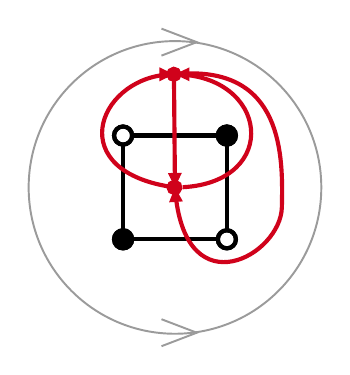
\begin{tikzpicture}[x=0.75pt,y=0.75pt,yscale=-1,xscale=1]
			%uncomment if require: \path (0,410); %set diagram left start at 0, and has height of 410
			
			%Shape: Circle [id:dp40869555012720693] 
			\draw  [color={rgb, 255:red, 155; green, 155; blue, 155 }  ,draw opacity=1 ][line width=0.7]  (266,186.5) .. controls (266,147.56) and (297.56,116) .. (336.5,116) .. controls (375.44,116) and (407,147.56) .. (407,186.5) .. controls (407,225.44) and (375.44,257) .. (336.5,257) .. controls (297.56,257) and (266,225.44) .. (266,186.5) -- cycle ;
            % Top >
			\draw  [color={rgb, 255:red, 155; green, 155; blue, 155 }  ,draw opacity=1 ][line width=0.7]  (330,110) -- (347,116.5) -- (330,123) ;
            % Bottom >
			\draw  [color={rgb, 255:red, 155; green, 155; blue, 155 }  ,draw opacity=1 ][line width=0.7]  (330,250) -- (347,256.5) -- (330,263) ;


			%Straight Lines [id:da4127487448285493] 
			\draw [line width=1.5]    (311.5,164.86) -- (311.5,211.5) ;
			\draw [shift={(311.5,211.5)}, rotate = 90] [color={rgb, 255:red, 0; green, 0; blue, 0 }  ][fill={rgb, 255:red, 0; green, 0; blue, 0 }  ][line width=1.5]      (0, 0) circle [x radius= 4.36, y radius= 4.36]   ;
			\draw [shift={(311.5,161.5)}, rotate = 90] [color={rgb, 255:red, 0; green, 0; blue, 0 }  ][line width=1.5]      (0, 0) circle [x radius= 4.36, y radius= 4.36]   ;
			%Straight Lines [id:da7856855933848323] 
			\draw [line width=1.5]    (358.15,211.5) -- (311.5,211.5) ;
			\draw [shift={(311.5,211.5)}, rotate = 180] [color={rgb, 255:red, 0; green, 0; blue, 0 }  ][fill={rgb, 255:red, 0; green, 0; blue, 0 }  ][line width=1.5]      (0, 0) circle [x radius= 4.36, y radius= 4.36]   ;
			\draw [shift={(361.5,211.5)}, rotate = 180] [color={rgb, 255:red, 0; green, 0; blue, 0 }  ][line width=1.5]      (0, 0) circle [x radius= 4.36, y radius= 4.36]   ;
			%Straight Lines [id:da9710750006314275] 
			\draw [line width=1.5]    (314.85,161.5) -- (361.5,161.5) ;
			\draw [shift={(361.5,161.5)}, rotate = 0] [color={rgb, 255:red, 0; green, 0; blue, 0 }  ][fill={rgb, 255:red, 0; green, 0; blue, 0 }  ][line width=1.5]      (0, 0) circle [x radius= 4.36, y radius= 4.36]   ;
			\draw [shift={(311.5,161.5)}, rotate = 0] [color={rgb, 255:red, 0; green, 0; blue, 0 }  ][line width=1.5]      (0, 0) circle [x radius= 4.36, y radius= 4.36]   ;
			%Straight Lines [id:da40578984072868207] 
			\draw [line width=1.5]    (361.5,208.15) -- (361.5,161.5) ;
			\draw [shift={(361.5,161.5)}, rotate = 270] [color={rgb, 255:red, 0; green, 0; blue, 0 }  ][fill={rgb, 255:red, 0; green, 0; blue, 0 }  ][line width=1.5]      (0, 0) circle [x radius= 4.36, y radius= 4.36]   ;
			\draw [shift={(361.5,211.5)}, rotate = 270] [color={rgb, 255:red, 0; green, 0; blue, 0 }  ][line width=1.5]      (0, 0) circle [x radius= 4.36, y radius= 4.36]   ;


			
			%Straight Lines [id:da9419202249102685] 
			\draw [color={rgb, 255:red, 208; green, 2; blue, 27 }  ,draw opacity=1 ][line width=1.5]    (336.46,182.5) -- (336,132) ;
			\draw [shift={(336,132)}, rotate = 269.47] [color={rgb, 255:red, 208; green, 2; blue, 27 }  ,draw opacity=1 ][fill={rgb, 255:red, 208; green, 2; blue, 27 }  ,fill opacity=1 ][line width=1.5]      (0, 0) circle [x radius= 2.61, y radius= 2.61]   ;
			\draw [shift={(336.5,186.5)}, rotate = 269.47] [fill={rgb, 255:red, 208; green, 2; blue, 27 }  ,fill opacity=1 ][line width=0.08]  [draw opacity=0] (6.97,-3.35) -- (0,0) -- (6.97,3.35) -- cycle    ;
			%Curve Lines [id:da9358575745335427] 
			\draw [color={rgb, 255:red, 208; green, 2; blue, 27 }  ,draw opacity=1 ][line width=1.5]    (336.5,186.5) .. controls (282.46,179.26) and (298.73,135.24) .. (332.28,132.17) ;
			\draw [shift={(336,132)}, rotate = 180] [fill={rgb, 255:red, 208; green, 2; blue, 27 }  ,fill opacity=1 ][line width=0.08]  [draw opacity=0] (6.97,-3.35) -- (0,0) -- (6.97,3.35) -- cycle    ;
			\draw [shift={(336.5,186.5)}, rotate = 187.63] [color={rgb, 255:red, 208; green, 2; blue, 27 }  ,draw opacity=1 ][fill={rgb, 255:red, 208; green, 2; blue, 27 }  ,fill opacity=1 ][line width=1.5]      (0, 0) circle [x radius= 2.61, y radius= 2.61]   ;
			%Curve Lines [id:da6328369708761336] 
			\draw [color={rgb, 255:red, 208; green, 2; blue, 27 }  ,draw opacity=1 ][line width=1.5]    (336,132) .. controls (381.83,132) and (387.72,183.81) .. (340.26,186.4) ;
			\draw [shift={(336.5,132)}, rotate = 360] [fill={rgb, 255:red, 208; green, 2; blue, 27 }  ,fill opacity=1 ][line width=0.08]  [draw opacity=0] (6.97,-3.35) -- (0,0) -- (6.97,3.35) -- cycle    ;
			\draw [shift={(336,186.5)}, rotate = 0] [color={rgb, 255:red, 208; green, 2; blue, 27 }  ,draw opacity=1 ][fill={rgb, 255:red, 208; green, 2; blue, 27 }  ,fill opacity=1 ][line width=1.5]      (0, 0) circle [x radius= 2.61, y radius= 2.61]   ;
			%Curve Lines [id:da7139538647060065] 
			\draw [color={rgb, 255:red, 208; green, 2; blue, 27 }  ,draw opacity=1 ][line width=1.5]    (336,132) .. controls (389.5,126.5) and (388.5,172.5) .. (388,196) .. controls (387.51,219.03) and (342.36,244.46) .. (336.79,189.94) ;
			\draw [shift={(336.5,186.5)}, rotate = 86.12] [fill={rgb, 255:red, 208; green, 2; blue, 27 }  ,fill opacity=1 ][line width=0.08]  [draw opacity=0] (6.97,-3.35) -- (0,0) -- (6.97,3.35) -- cycle    ;
			\draw [shift={(336,132)}, rotate = 354.13] [color={rgb, 255:red, 208; green, 2; blue, 27 }  ,draw opacity=1 ][fill={rgb, 255:red, 208; green, 2; blue, 27 }  ,fill opacity=1 ][line width=1.5]      (0, 0) circle [x radius= 2.61, y radius= 2.61]   ;
		\end{tikzpicture}
	\end{center}
    Multiple $2$-cycles above. Mutating non-cluster quivers not allowed!
\end{frame}

\begin{frame}{Quivers with Potential}
    \textbf{Potential} of a dimer quiver $Q$ is the formal quantity \cite{bocklandtDimerABC2015}
    \begin{align*}
        W = \sum (\text{cycles of } Q \text{ about } \bullet) - \sum (\text{cycles of } Q \text{ about } \circ).
    \end{align*}
    Cycles are determined up to cyclical equivalence: $abc$ is equivalent to $bca$.
    \begin{itemize}
        \justifying
        \item Rigorously defined using path algebras: $W$ is an element of the quotient space $\CC Q/[\CC Q, \CC Q]$ where $[\CC Q, \CC Q]$ is the subspace of $\CC Q$ spanned by commutators.
        \begin{itemize}
            \item A way for representation theory to enter the picture! We will ignore this perspective entirely, though :(
        \end{itemize}
    \end{itemize}
    The pair $(Q, W)$ is called a \textbf{quiver with potential} \cite{derksenQuiversPotentialsTheir2007}.
\end{frame}

\begin{frame}{Example}
    Example of computing potential of following dimer on sphere:
	\begin{center}
		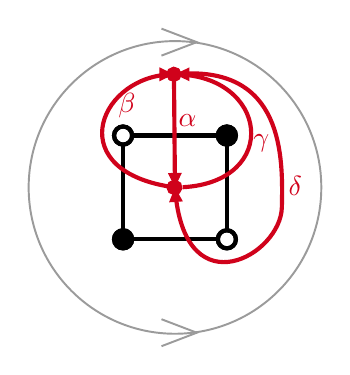
\begin{tikzpicture}[x=0.75pt,y=0.75pt,yscale=-1,xscale=1]
			%uncomment if require: \path (0,410); %set diagram left start at 0, and has height of 410
			
			%Shape: Circle [id:dp40869555012720693] 
			\draw  [color={rgb, 255:red, 155; green, 155; blue, 155 }  ,draw opacity=1 ][line width=0.7]  (266,186.5) .. controls (266,147.56) and (297.56,116) .. (336.5,116) .. controls (375.44,116) and (407,147.56) .. (407,186.5) .. controls (407,225.44) and (375.44,257) .. (336.5,257) .. controls (297.56,257) and (266,225.44) .. (266,186.5) -- cycle ;
            % Top >
			\draw  [color={rgb, 255:red, 155; green, 155; blue, 155 }  ,draw opacity=1 ][line width=0.7]  (330,110) -- (347,116.5) -- (330,123) ;
            % Bottom >
			\draw  [color={rgb, 255:red, 155; green, 155; blue, 155 }  ,draw opacity=1 ][line width=0.7]  (330,250) -- (347,256.5) -- (330,263) ;


			%Straight Lines [id:da4127487448285493] 
			\draw [line width=1.5]    (311.5,164.86) -- (311.5,211.5) ;
			\draw [shift={(311.5,211.5)}, rotate = 90] [color={rgb, 255:red, 0; green, 0; blue, 0 }  ][fill={rgb, 255:red, 0; green, 0; blue, 0 }  ][line width=1.5]      (0, 0) circle [x radius= 4.36, y radius= 4.36]   ;
			\draw [shift={(311.5,161.5)}, rotate = 90] [color={rgb, 255:red, 0; green, 0; blue, 0 }  ][line width=1.5]      (0, 0) circle [x radius= 4.36, y radius= 4.36]   ;
			%Straight Lines [id:da7856855933848323] 
			\draw [line width=1.5]    (358.15,211.5) -- (311.5,211.5) ;
			\draw [shift={(311.5,211.5)}, rotate = 180] [color={rgb, 255:red, 0; green, 0; blue, 0 }  ][fill={rgb, 255:red, 0; green, 0; blue, 0 }  ][line width=1.5]      (0, 0) circle [x radius= 4.36, y radius= 4.36]   ;
			\draw [shift={(361.5,211.5)}, rotate = 180] [color={rgb, 255:red, 0; green, 0; blue, 0 }  ][line width=1.5]      (0, 0) circle [x radius= 4.36, y radius= 4.36]   ;
			%Straight Lines [id:da9710750006314275] 
			\draw [line width=1.5]    (314.85,161.5) -- (361.5,161.5) ;
			\draw [shift={(361.5,161.5)}, rotate = 0] [color={rgb, 255:red, 0; green, 0; blue, 0 }  ][fill={rgb, 255:red, 0; green, 0; blue, 0 }  ][line width=1.5]      (0, 0) circle [x radius= 4.36, y radius= 4.36]   ;
			\draw [shift={(311.5,161.5)}, rotate = 0] [color={rgb, 255:red, 0; green, 0; blue, 0 }  ][line width=1.5]      (0, 0) circle [x radius= 4.36, y radius= 4.36]   ;
			%Straight Lines [id:da40578984072868207] 
			\draw [line width=1.5]    (361.5,208.15) -- (361.5,161.5) ;
			\draw [shift={(361.5,161.5)}, rotate = 270] [color={rgb, 255:red, 0; green, 0; blue, 0 }  ][fill={rgb, 255:red, 0; green, 0; blue, 0 }  ][line width=1.5]      (0, 0) circle [x radius= 4.36, y radius= 4.36]   ;
			\draw [shift={(361.5,211.5)}, rotate = 270] [color={rgb, 255:red, 0; green, 0; blue, 0 }  ][line width=1.5]      (0, 0) circle [x radius= 4.36, y radius= 4.36]   ;


			
			%Straight Lines [id:da9419202249102685] 
			\draw [color={rgb, 255:red, 208; green, 2; blue, 27 }  ,draw opacity=1 ][line width=1.5]    (336.46,182.5) -- (336,132) ;
			\draw [shift={(336,132)}, rotate = 269.47] [color={rgb, 255:red, 208; green, 2; blue, 27 }  ,draw opacity=1 ][fill={rgb, 255:red, 208; green, 2; blue, 27 }  ,fill opacity=1 ][line width=1.5]      (0, 0) circle [x radius= 2.61, y radius= 2.61]   ;
			\draw [shift={(336.5,186.5)}, rotate = 269.47] [fill={rgb, 255:red, 208; green, 2; blue, 27 }  ,fill opacity=1 ][line width=0.08]  [draw opacity=0] (6.97,-3.35) -- (0,0) -- (6.97,3.35) -- cycle    ;
			%Curve Lines [id:da9358575745335427] 
			\draw [color={rgb, 255:red, 208; green, 2; blue, 27 }  ,draw opacity=1 ][line width=1.5]    (336.5,186.5) .. controls (282.46,179.26) and (298.73,135.24) .. (332.28,132.17) ;
			\draw [shift={(336,132)}, rotate = 180] [fill={rgb, 255:red, 208; green, 2; blue, 27 }  ,fill opacity=1 ][line width=0.08]  [draw opacity=0] (6.97,-3.35) -- (0,0) -- (6.97,3.35) -- cycle    ;
			\draw [shift={(336.5,186.5)}, rotate = 187.63] [color={rgb, 255:red, 208; green, 2; blue, 27 }  ,draw opacity=1 ][fill={rgb, 255:red, 208; green, 2; blue, 27 }  ,fill opacity=1 ][line width=1.5]      (0, 0) circle [x radius= 2.61, y radius= 2.61]   ;
			%Curve Lines [id:da6328369708761336] 
			\draw [color={rgb, 255:red, 208; green, 2; blue, 27 }  ,draw opacity=1 ][line width=1.5]    (336,132) .. controls (381.83,132) and (387.72,183.81) .. (340.26,186.4) ;
			\draw [shift={(336.5,132)}, rotate = 360] [fill={rgb, 255:red, 208; green, 2; blue, 27 }  ,fill opacity=1 ][line width=0.08]  [draw opacity=0] (6.97,-3.35) -- (0,0) -- (6.97,3.35) -- cycle    ;
			\draw [shift={(336,186.5)}, rotate = 0] [color={rgb, 255:red, 208; green, 2; blue, 27 }  ,draw opacity=1 ][fill={rgb, 255:red, 208; green, 2; blue, 27 }  ,fill opacity=1 ][line width=1.5]      (0, 0) circle [x radius= 2.61, y radius= 2.61]   ;
			%Curve Lines [id:da7139538647060065] 
			\draw [color={rgb, 255:red, 208; green, 2; blue, 27 }  ,draw opacity=1 ][line width=1.5]    (336,132) .. controls (389.5,126.5) and (388.5,172.5) .. (388,196) .. controls (387.51,219.03) and (342.36,244.46) .. (336.79,189.94) ;
			\draw [shift={(336.5,186.5)}, rotate = 86.12] [fill={rgb, 255:red, 208; green, 2; blue, 27 }  ,fill opacity=1 ][line width=0.08]  [draw opacity=0] (6.97,-3.35) -- (0,0) -- (6.97,3.35) -- cycle    ;
			\draw [shift={(336,132)}, rotate = 354.13] [color={rgb, 255:red, 208; green, 2; blue, 27 }  ,draw opacity=1 ][fill={rgb, 255:red, 208; green, 2; blue, 27 }  ,fill opacity=1 ][line width=1.5]      (0, 0) circle [x radius= 2.61, y radius= 2.61]   ;
			
			
			\draw (337, 150) node [anchor=north west][inner sep=0.75pt] [align=left] {$\displaystyle \textcolor[rgb]{0.82,0.01,0.11}{\alpha}$};
			\draw (308, 140) node [anchor=north west][inner sep=0.75pt] [align=left] {$\displaystyle \textcolor[rgb]{0.82,0.01,0.11}{\beta}$};
			\draw (373, 160) node [anchor=north west][inner sep=0.75pt] [align=left] {$\displaystyle \textcolor[rgb]{0.82,0.01,0.11}{\gamma}$};
			\draw (390, 180) node [anchor=north west][inner sep=0.75pt] [align=left] {$\displaystyle \textcolor[rgb]{0.82,0.01,0.11}{\delta}$};
			\end{tikzpicture}
	\end{center}
	Here $W = \alpha\gamma + \beta\delta - \alpha\beta - \gamma\delta$
\end{frame}

\begin{frame}{Mutation of Quivers with Potential}
Recall steps of quiver mutation:
\begin{enumerate}
    \item For each path $v \to x \to w$, add a new arrow $v \to w$
    \item Reverse orientation of arrows incident to $x$
    \item Remove any pairs of arrows forming $2$-cycles. Repeat until no more $2$-cycles are left
\end{enumerate}
To \textbf{mutate} $(Q, W)$, modify step 1 to add newly created cycles to $W$ and step 3 to only delete $2$-cycles that are in $W$. The resultant quiver is denoted $\mu_x(Q, W)$.

\vspace{0.5cm}

This modified variant is known as \textbf{QP mutation} as described by Derksen, Weyman, and Zelevinsky \cite{derksenQuiversPotentialsTheir2007}. The potential allows us to control which $2$-cycles are allowed to be deleted and which are left alone.
\end{frame}

\begin{frame}{Join Moves}
    Here, we introduce the dimer equivalent of deleting $2$-cycles from the quiver.

    \vspace{0.5cm}

    A \textbf{join move} removes a degree-$2$ (bivalent) node of a dimer model and joins the two nodes connected to it.
	\begin{center}
		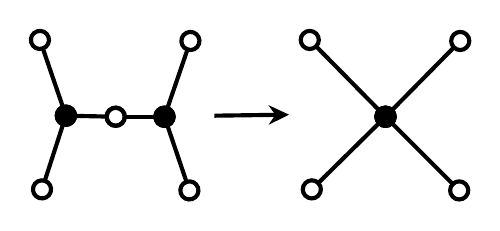
\begin{tikzpicture}[x=0.75pt,y=0.75pt,yscale=-1,xscale=1]
			%uncomment if require: \path (0,410); %set diagram left start at 0, and has height of 410
			
			%Straight Lines [id:da3213994062019696] 
			\draw [line width=1.5]    (120.5,108.5) -- (141.15,108.93) ;
			\draw [shift={(144.5,109)}, rotate = 1.19] [color={rgb, 255:red, 0; green, 0; blue, 0 }  ][line width=1.5]      (0, 0) circle [x radius= 4.36, y radius= 4.36]   ;
			\draw [shift={(120.5,108.5)}, rotate = 1.19] [color={rgb, 255:red, 0; green, 0; blue, 0 }  ][fill={rgb, 255:red, 0; green, 0; blue, 0 }  ][line width=1.5]      (0, 0) circle [x radius= 4.36, y radius= 4.36]   ;
			%Straight Lines [id:da6871882433843249] 
			\draw [line width=1.5]    (168,109) -- (147.85,109) ;
			\draw [shift={(144.5,109)}, rotate = 180] [color={rgb, 255:red, 0; green, 0; blue, 0 }  ][line width=1.5]      (0, 0) circle [x radius= 4.36, y radius= 4.36]   ;
			\draw [shift={(168,109)}, rotate = 180] [color={rgb, 255:red, 0; green, 0; blue, 0 }  ][fill={rgb, 255:red, 0; green, 0; blue, 0 }  ][line width=1.5]      (0, 0) circle [x radius= 4.36, y radius= 4.36]   ;
			%Straight Lines [id:da9688852471034756] 
			\draw [line width=1.5]    (168,109) -- (179.41,75.67) ;
			\draw [shift={(180.5,72.5)}, rotate = 288.9] [color={rgb, 255:red, 0; green, 0; blue, 0 }  ][line width=1.5]      (0, 0) circle [x radius= 4.36, y radius= 4.36]   ;
			\draw [shift={(168,109)}, rotate = 288.9] [color={rgb, 255:red, 0; green, 0; blue, 0 }  ][fill={rgb, 255:red, 0; green, 0; blue, 0 }  ][line width=1.5]      (0, 0) circle [x radius= 4.36, y radius= 4.36]   ;
			%Straight Lines [id:da7180372925711271] 
			\draw [line width=1.5]    (168,109) -- (178.93,141.32) ;
			\draw [shift={(180,144.5)}, rotate = 71.32] [color={rgb, 255:red, 0; green, 0; blue, 0 }  ][line width=1.5]      (0, 0) circle [x radius= 4.36, y radius= 4.36]   ;
			\draw [shift={(168,109)}, rotate = 71.32] [color={rgb, 255:red, 0; green, 0; blue, 0 }  ][fill={rgb, 255:red, 0; green, 0; blue, 0 }  ][line width=1.5]      (0, 0) circle [x radius= 4.36, y radius= 4.36]   ;
			%Straight Lines [id:da7066959168241529] 
			\draw [line width=1.5]    (120.5,108.5) -- (109.09,75.17) ;
			\draw [shift={(108,72)}, rotate = 251.1] [color={rgb, 255:red, 0; green, 0; blue, 0 }  ][line width=1.5]      (0, 0) circle [x radius= 4.36, y radius= 4.36]   ;
			\draw [shift={(120.5,108.5)}, rotate = 251.1] [color={rgb, 255:red, 0; green, 0; blue, 0 }  ][fill={rgb, 255:red, 0; green, 0; blue, 0 }  ][line width=1.5]      (0, 0) circle [x radius= 4.36, y radius= 4.36]   ;
			%Straight Lines [id:da1350258580761733] 
			\draw [line width=1.5]    (120.5,108.5) -- (110.03,140.81) ;
			\draw [shift={(109,144)}, rotate = 107.95] [color={rgb, 255:red, 0; green, 0; blue, 0 }  ][line width=1.5]      (0, 0) circle [x radius= 4.36, y radius= 4.36]   ;
			\draw [shift={(120.5,108.5)}, rotate = 107.95] [color={rgb, 255:red, 0; green, 0; blue, 0 }  ][fill={rgb, 255:red, 0; green, 0; blue, 0 }  ][line width=1.5]      (0, 0) circle [x radius= 4.36, y radius= 4.36]   ;
			%Straight Lines [id:da8946693699424726] 
			\draw [line width=1.5]    (274.5,109) ;
			\draw [shift={(274.5,109)}, rotate = 0] [color={rgb, 255:red, 0; green, 0; blue, 0 }  ][line width=1.5]      (0, 0) circle [x radius= 4.36, y radius= 4.36]   ;
			\draw [shift={(274.5,109)}, rotate = 0] [color={rgb, 255:red, 0; green, 0; blue, 0 }  ][fill={rgb, 255:red, 0; green, 0; blue, 0 }  ][line width=1.5]      (0, 0) circle [x radius= 4.36, y radius= 4.36]   ;
			%Straight Lines [id:da037487795586125805] 
			\draw [line width=1.5]    (274.5,109) ;
			\draw [shift={(274.5,109)}, rotate = 0] [color={rgb, 255:red, 0; green, 0; blue, 0 }  ][line width=1.5]      (0, 0) circle [x radius= 4.36, y radius= 4.36]   ;
			\draw [shift={(274.5,109)}, rotate = 0] [color={rgb, 255:red, 0; green, 0; blue, 0 }  ][fill={rgb, 255:red, 0; green, 0; blue, 0 }  ][line width=1.5]      (0, 0) circle [x radius= 4.36, y radius= 4.36]   ;
			%Straight Lines [id:da5216750978884044] 
			\draw [line width=1.5]    (274.5,109) -- (308.14,74.89) ;
			\draw [shift={(310.5,72.5)}, rotate = 314.6] [color={rgb, 255:red, 0; green, 0; blue, 0 }  ][line width=1.5]      (0, 0) circle [x radius= 4.36, y radius= 4.36]   ;
			%Straight Lines [id:da060862821009733836] 
			\draw [line width=1.5]    (274.5,109) -- (307.63,142.13) ;
			\draw [shift={(310,144.5)}, rotate = 45] [color={rgb, 255:red, 0; green, 0; blue, 0 }  ][line width=1.5]      (0, 0) circle [x radius= 4.36, y radius= 4.36]   ;
			%Straight Lines [id:da5106533762297103] 
			\draw [line width=1.5]    (274.5,109) -- (240.36,74.39) ;
			\draw [shift={(238,72)}, rotate = 225.39] [color={rgb, 255:red, 0; green, 0; blue, 0 }  ][line width=1.5]      (0, 0) circle [x radius= 4.36, y radius= 4.36]   ;
			%Straight Lines [id:da084201108785671] 
			\draw [line width=1.5]    (274.5,109) -- (241.39,141.64) ;
			\draw [shift={(239,144)}, rotate = 135.41] [color={rgb, 255:red, 0; green, 0; blue, 0 }  ][line width=1.5]      (0, 0) circle [x radius= 4.36, y radius= 4.36]   ;
			%Straight Lines [id:da993073009551671] 
			\draw [line width=1.5]    (192,108.5) -- (224,108.06) ;
			\draw [shift={(228,108)}, rotate = 179.2] [fill={rgb, 255:red, 0; green, 0; blue, 0 }  ][line width=0.08]  [draw opacity=0] (9.91,-4.76) -- (0,0) -- (9.91,4.76) -- (6.58,0) -- cycle    ;
		\end{tikzpicture}			
	\end{center}
\end{frame}

\begin{frame}{Dimer Models and QP Mutation}
    We motivate (a special case of) dimer model version of QP mutation using QP mutation.
    \begin{center}
        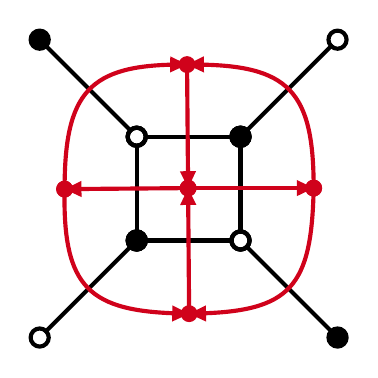
\begin{tikzpicture}[x=0.75pt,y=0.75pt,yscale=-1,xscale=1]
            %uncomment if require: \path (0,410); %set diagram left start at 0, and has height of 410
            
            %Straight Lines [id:da005183270613696722] 
            \draw [line width=1.5]    (168.5,48.5) -- (212.88,92.88) ;
            \draw [shift={(215.25,95.25)}, rotate = 45] [color={rgb, 255:red, 0; green, 0; blue, 0 }  ][line width=1.5]      (0, 0) circle [x radius= 4.36, y radius= 4.36]   ;
            \draw [shift={(168.5,48.5)}, rotate = 45] [color={rgb, 255:red, 0; green, 0; blue, 0 }  ][fill={rgb, 255:red, 0; green, 0; blue, 0 }  ][line width=1.5]      (0, 0) circle [x radius= 4.36, y radius= 4.36]   ;
            %Straight Lines [id:da3934001790859082] 
            \draw [line width=1.5]    (265.25,95.25) -- (218.61,95.25) ;
            \draw [shift={(215.25,95.25)}, rotate = 180] [color={rgb, 255:red, 0; green, 0; blue, 0 }  ][line width=1.5]      (0, 0) circle [x radius= 4.36, y radius= 4.36]   ;
            \draw [shift={(265.25,95.25)}, rotate = 180] [color={rgb, 255:red, 0; green, 0; blue, 0 }  ][fill={rgb, 255:red, 0; green, 0; blue, 0 }  ][line width=1.5]      (0, 0) circle [x radius= 4.36, y radius= 4.36]   ;
            %Straight Lines [id:da9659933453892754] 
            \draw [line width=1.5]    (265.25,95.25) -- (265.25,141.9) ;
            \draw [shift={(265.25,145.25)}, rotate = 90] [color={rgb, 255:red, 0; green, 0; blue, 0 }  ][line width=1.5]      (0, 0) circle [x radius= 4.36, y radius= 4.36]   ;
            \draw [shift={(265.25,95.25)}, rotate = 90] [color={rgb, 255:red, 0; green, 0; blue, 0 }  ][fill={rgb, 255:red, 0; green, 0; blue, 0 }  ][line width=1.5]      (0, 0) circle [x radius= 4.36, y radius= 4.36]   ;
            %Straight Lines [id:da9529887421615183] 
            \draw [line width=1.5]    (215.25,145.25) -- (261.9,145.25) ;
            \draw [shift={(265.25,145.25)}, rotate = 0] [color={rgb, 255:red, 0; green, 0; blue, 0 }  ][line width=1.5]      (0, 0) circle [x radius= 4.36, y radius= 4.36]   ;
            \draw [shift={(215.25,145.25)}, rotate = 0] [color={rgb, 255:red, 0; green, 0; blue, 0 }  ][fill={rgb, 255:red, 0; green, 0; blue, 0 }  ][line width=1.5]      (0, 0) circle [x radius= 4.36, y radius= 4.36]   ;
            %Straight Lines [id:da4731035021017006] 
            \draw [line width=1.5]    (215.25,145.25) -- (215.25,98.61) ;
            \draw [shift={(215.25,95.25)}, rotate = 270] [color={rgb, 255:red, 0; green, 0; blue, 0 }  ][line width=1.5]      (0, 0) circle [x radius= 4.36, y radius= 4.36]   ;
            \draw [shift={(215.25,145.25)}, rotate = 270] [color={rgb, 255:red, 0; green, 0; blue, 0 }  ][fill={rgb, 255:red, 0; green, 0; blue, 0 }  ][line width=1.5]      (0, 0) circle [x radius= 4.36, y radius= 4.36]   ;
            %Straight Lines [id:da7035573274275309] 
            \draw [line width=1.5]    (312,192) -- (267.62,147.62) ;
            \draw [shift={(265.25,145.25)}, rotate = 225] [color={rgb, 255:red, 0; green, 0; blue, 0 }  ][line width=1.5]      (0, 0) circle [x radius= 4.36, y radius= 4.36]   ;
            \draw [shift={(312,192)}, rotate = 225] [color={rgb, 255:red, 0; green, 0; blue, 0 }  ][fill={rgb, 255:red, 0; green, 0; blue, 0 }  ][line width=1.5]      (0, 0) circle [x radius= 4.36, y radius= 4.36]   ;
            %Straight Lines [id:da2333804230649933] 
            \draw [line width=1.5]    (265.25,95.25) -- (309.63,50.87) ;
            \draw [shift={(312,48.5)}, rotate = 315] [color={rgb, 255:red, 0; green, 0; blue, 0 }  ][line width=1.5]      (0, 0) circle [x radius= 4.36, y radius= 4.36]   ;
            \draw [shift={(265.25,95.25)}, rotate = 315] [color={rgb, 255:red, 0; green, 0; blue, 0 }  ][fill={rgb, 255:red, 0; green, 0; blue, 0 }  ][line width=1.5]      (0, 0) circle [x radius= 4.36, y radius= 4.36]   ;
            %Straight Lines [id:da9003382621189856] 
            \draw [line width=1.5]    (215.25,145.25) -- (170.87,189.63) ;
            \draw [shift={(168.5,192)}, rotate = 135] [color={rgb, 255:red, 0; green, 0; blue, 0 }  ][line width=1.5]      (0, 0) circle [x radius= 4.36, y radius= 4.36]   ;
            \draw [shift={(215.25,145.25)}, rotate = 135] [color={rgb, 255:red, 0; green, 0; blue, 0 }  ][fill={rgb, 255:red, 0; green, 0; blue, 0 }  ][line width=1.5]      (0, 0) circle [x radius= 4.36, y radius= 4.36]   ;
            %Straight Lines [id:da46853719520681536] 
            \draw [color={rgb, 255:red, 208; green, 2; blue, 27 }  ,draw opacity=1 ][line width=1.5]    (240,120) -- (184.5,120.47) ;
            \draw [shift={(180.5,120.5)}, rotate = 359.52] [fill={rgb, 255:red, 208; green, 2; blue, 27 }  ,fill opacity=1 ][line width=0.08]  [draw opacity=0] (8.13,-3.9) -- (0,0) -- (8.13,3.9) -- cycle    ;
            \draw [shift={(240,120)}, rotate = 179.52] [color={rgb, 255:red, 208; green, 2; blue, 27 }  ,draw opacity=1 ][fill={rgb, 255:red, 208; green, 2; blue, 27 }  ,fill opacity=1 ][line width=1.5]      (0, 0) circle [x radius= 3.05, y radius= 3.05]   ;
            %Straight Lines [id:da61878858835384] 
            \draw [color={rgb, 255:red, 208; green, 2; blue, 27 }  ,draw opacity=1 ][line width=1.5]    (240.5,180.5) -- (240.03,124) ;
            \draw [shift={(240,120)}, rotate = 89.53] [fill={rgb, 255:red, 208; green, 2; blue, 27 }  ,fill opacity=1 ][line width=0.08]  [draw opacity=0] (8.13,-3.9) -- (0,0) -- (8.13,3.9) -- cycle    ;
            \draw [shift={(240.5,180.5)}, rotate = 269.53] [color={rgb, 255:red, 208; green, 2; blue, 27 }  ,draw opacity=1 ][fill={rgb, 255:red, 208; green, 2; blue, 27 }  ,fill opacity=1 ][line width=1.5]      (0, 0) circle [x radius= 3.05, y radius= 3.05]   ;
            %Straight Lines [id:da4629638495700332] 
            \draw [color={rgb, 255:red, 208; green, 2; blue, 27 }  ,draw opacity=1 ][line width=1.5]    (240,120) -- (296.5,120) ;
            \draw [shift={(300.5,120)}, rotate = 180] [fill={rgb, 255:red, 208; green, 2; blue, 27 }  ,fill opacity=1 ][line width=0.08]  [draw opacity=0] (8.13,-3.9) -- (0,0) -- (8.13,3.9) -- cycle    ;
            \draw [shift={(240,120)}, rotate = 0] [color={rgb, 255:red, 208; green, 2; blue, 27 }  ,draw opacity=1 ][fill={rgb, 255:red, 208; green, 2; blue, 27 }  ,fill opacity=1 ][line width=1.5]      (0, 0) circle [x radius= 3.05, y radius= 3.05]   ;
            %Straight Lines [id:da8207445621825815] 
            \draw [color={rgb, 255:red, 208; green, 2; blue, 27 }  ,draw opacity=1 ][line width=1.5]    (239.5,60.5) -- (239.97,116) ;
            \draw [shift={(240,120)}, rotate = 269.52] [fill={rgb, 255:red, 208; green, 2; blue, 27 }  ,fill opacity=1 ][line width=0.08]  [draw opacity=0] (8.13,-3.9) -- (0,0) -- (8.13,3.9) -- cycle    ;
            \draw [shift={(239.5,60.5)}, rotate = 89.52] [color={rgb, 255:red, 208; green, 2; blue, 27 }  ,draw opacity=1 ][fill={rgb, 255:red, 208; green, 2; blue, 27 }  ,fill opacity=1 ][line width=1.5]      (0, 0) circle [x radius= 3.05, y radius= 3.05]   ;
            %Curve Lines [id:da6522412714275189] 
            \draw [color={rgb, 255:red, 208; green, 2; blue, 27 }  ,draw opacity=1 ][line width=1.5]    (180.5,120.5) .. controls (180.5,73.7) and (192.38,60.65) .. (236.08,60.49) ;
            \draw [shift={(239.5,60.5)}, rotate = 180.62] [fill={rgb, 255:red, 208; green, 2; blue, 27 }  ,fill opacity=1 ][line width=0.08]  [draw opacity=0] (8.13,-3.9) -- (0,0) -- (8.13,3.9) -- cycle    ;
            \draw [shift={(180.5,120.5)}, rotate = 270] [color={rgb, 255:red, 208; green, 2; blue, 27 }  ,draw opacity=1 ][fill={rgb, 255:red, 208; green, 2; blue, 27 }  ,fill opacity=1 ][line width=1.5]      (0, 0) circle [x radius= 3.05, y radius= 3.05]   ;
            %Curve Lines [id:da6991631851136911] 
            \draw [color={rgb, 255:red, 208; green, 2; blue, 27 }  ,draw opacity=1 ][line width=1.5]    (300.5,120) .. controls (300.5,73.2) and (288.62,60.62) .. (243.07,60.49) ;
            \draw [shift={(239.5,60.5)}, rotate = 359.41] [fill={rgb, 255:red, 208; green, 2; blue, 27 }  ,fill opacity=1 ][line width=0.08]  [draw opacity=0] (8.13,-3.9) -- (0,0) -- (8.13,3.9) -- cycle    ;
            \draw [shift={(300.5,120)}, rotate = 270] [color={rgb, 255:red, 208; green, 2; blue, 27 }  ,draw opacity=1 ][fill={rgb, 255:red, 208; green, 2; blue, 27 }  ,fill opacity=1 ][line width=1.5]      (0, 0) circle [x radius= 3.05, y radius= 3.05]   ;
            %Curve Lines [id:da05762502854813123] 
            \draw [color={rgb, 255:red, 208; green, 2; blue, 27 }  ,draw opacity=1 ][line width=1.5]    (300.5,120) .. controls (299.52,167.78) and (289.52,179.43) .. (244.07,180.44) ;
            \draw [shift={(240.5,180.5)}, rotate = 359.41] [fill={rgb, 255:red, 208; green, 2; blue, 27 }  ,fill opacity=1 ][line width=0.08]  [draw opacity=0] (8.13,-3.9) -- (0,0) -- (8.13,3.9) -- cycle    ;
            \draw [shift={(300.5,120)}, rotate = 91.17] [color={rgb, 255:red, 208; green, 2; blue, 27 }  ,draw opacity=1 ][fill={rgb, 255:red, 208; green, 2; blue, 27 }  ,fill opacity=1 ][line width=1.5]      (0, 0) circle [x radius= 3.05, y radius= 3.05]   ;
            %Curve Lines [id:da4220575863684264] 
            \draw [color={rgb, 255:red, 208; green, 2; blue, 27 }  ,draw opacity=1 ][line width=1.5]    (180.5,120.5) .. controls (179.53,168.28) and (192.33,179.45) .. (237,180.44) ;
            \draw [shift={(240.5,180.5)}, rotate = 180.6] [fill={rgb, 255:red, 208; green, 2; blue, 27 }  ,fill opacity=1 ][line width=0.08]  [draw opacity=0] (8.13,-3.9) -- (0,0) -- (8.13,3.9) -- cycle    ;
            \draw [shift={(180.5,120.5)}, rotate = 91.17] [color={rgb, 255:red, 208; green, 2; blue, 27 }  ,draw opacity=1 ][fill={rgb, 255:red, 208; green, 2; blue, 27 }  ,fill opacity=1 ][line width=1.5]      (0, 0) circle [x radius= 3.05, y radius= 3.05]   ;
            \end{tikzpicture}
    \end{center}
    We will do QP mutation on the center vertex of the quiver.
\end{frame}

\begin{frame}{Dimer Models and QP Mutation (cont.)}
    Steps 1 and 2 of QP mutation:
    \begin{center}
        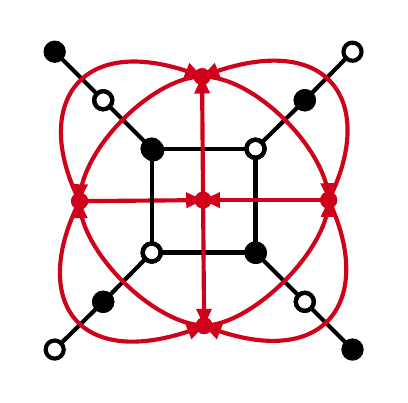
\begin{tikzpicture}[x=0.75pt,y=0.75pt,yscale=-1,xscale=1]
            %uncomment if require: \path (0,410); %set diagram left start at 0, and has height of 410
            
            %Straight Lines [id:da005183270613696722] 
            \draw [line width=1.5]    (168.5,48.5) -- (189.5,69.5) ;
            \draw [shift={(191.88,71.88)}, rotate = 45] [color={rgb, 255:red, 0; green, 0; blue, 0 }  ][line width=1.5]      (0, 0) circle [x radius= 4.36, y radius= 4.36]   ;
            \draw [shift={(168.5,48.5)}, rotate = 45] [color={rgb, 255:red, 0; green, 0; blue, 0 }  ][fill={rgb, 255:red, 0; green, 0; blue, 0 }  ][line width=1.5]      (0, 0) circle [x radius= 4.36, y radius= 4.36]   ;
            %Straight Lines [id:da3934001790859082] 
            \draw [line width=1.5]    (261.9,95.25) -- (215.25,95.25) ;
            \draw [shift={(215.25,95.25)}, rotate = 180] [color={rgb, 255:red, 0; green, 0; blue, 0 }  ][fill={rgb, 255:red, 0; green, 0; blue, 0 }  ][line width=1.5]      (0, 0) circle [x radius= 4.36, y radius= 4.36]   ;
            \draw [shift={(265.25,95.25)}, rotate = 180] [color={rgb, 255:red, 0; green, 0; blue, 0 }  ][line width=1.5]      (0, 0) circle [x radius= 4.36, y radius= 4.36]   ;
            %Straight Lines [id:da9659933453892754] 
            \draw [line width=1.5]    (265.25,98.6) -- (265.25,145.25) ;
            \draw [shift={(265.25,145.25)}, rotate = 90] [color={rgb, 255:red, 0; green, 0; blue, 0 }  ][fill={rgb, 255:red, 0; green, 0; blue, 0 }  ][line width=1.5]      (0, 0) circle [x radius= 4.36, y radius= 4.36]   ;
            \draw [shift={(265.25,95.25)}, rotate = 90] [color={rgb, 255:red, 0; green, 0; blue, 0 }  ][line width=1.5]      (0, 0) circle [x radius= 4.36, y radius= 4.36]   ;
            %Straight Lines [id:da9529887421615183] 
            \draw [line width=1.5]    (218.61,145.25) -- (265.25,145.25) ;
            \draw [shift={(265.25,145.25)}, rotate = 0] [color={rgb, 255:red, 0; green, 0; blue, 0 }  ][fill={rgb, 255:red, 0; green, 0; blue, 0 }  ][line width=1.5]      (0, 0) circle [x radius= 4.36, y radius= 4.36]   ;
            \draw [shift={(215.25,145.25)}, rotate = 0] [color={rgb, 255:red, 0; green, 0; blue, 0 }  ][line width=1.5]      (0, 0) circle [x radius= 4.36, y radius= 4.36]   ;
            %Straight Lines [id:da7035573274275309] 
            \draw [line width=1.5]    (312,192) -- (291.37,171.37) ;
            \draw [shift={(289,169)}, rotate = 225] [color={rgb, 255:red, 0; green, 0; blue, 0 }  ][line width=1.5]      (0, 0) circle [x radius= 4.36, y radius= 4.36]   ;
            \draw [shift={(312,192)}, rotate = 225] [color={rgb, 255:red, 0; green, 0; blue, 0 }  ][fill={rgb, 255:red, 0; green, 0; blue, 0 }  ][line width=1.5]      (0, 0) circle [x radius= 4.36, y radius= 4.36]   ;
            %Straight Lines [id:da2333804230649933] 
            \draw [line width=1.5]    (289,71.88) -- (309.65,50.89) ;
            \draw [shift={(312,48.5)}, rotate = 314.54] [color={rgb, 255:red, 0; green, 0; blue, 0 }  ][line width=1.5]      (0, 0) circle [x radius= 4.36, y radius= 4.36]   ;
            \draw [shift={(289,71.88)}, rotate = 314.54] [color={rgb, 255:red, 0; green, 0; blue, 0 }  ][fill={rgb, 255:red, 0; green, 0; blue, 0 }  ][line width=1.5]      (0, 0) circle [x radius= 4.36, y radius= 4.36]   ;
            %Straight Lines [id:da9003382621189856] 
            \draw [line width=1.5]    (191.88,169) -- (170.89,189.65) ;
            \draw [shift={(168.5,192)}, rotate = 135.46] [color={rgb, 255:red, 0; green, 0; blue, 0 }  ][line width=1.5]      (0, 0) circle [x radius= 4.36, y radius= 4.36]   ;
            \draw [shift={(191.88,169)}, rotate = 135.46] [color={rgb, 255:red, 0; green, 0; blue, 0 }  ][fill={rgb, 255:red, 0; green, 0; blue, 0 }  ][line width=1.5]      (0, 0) circle [x radius= 4.36, y radius= 4.36]   ;
            %Straight Lines [id:da46853719520681536] 
            \draw [color={rgb, 255:red, 208; green, 2; blue, 27 }  ,draw opacity=1 ][line width=1.5]    (236,120.03) -- (180.5,120.5) ;
            \draw [shift={(180.5,120.5)}, rotate = 179.52] [color={rgb, 255:red, 208; green, 2; blue, 27 }  ,draw opacity=1 ][fill={rgb, 255:red, 208; green, 2; blue, 27 }  ,fill opacity=1 ][line width=1.5]      (0, 0) circle [x radius= 3.05, y radius= 3.05]   ;
            \draw [shift={(240,120)}, rotate = 179.52] [fill={rgb, 255:red, 208; green, 2; blue, 27 }  ,fill opacity=1 ][line width=0.08]  [draw opacity=0] (8.13,-3.9) -- (0,0) -- (8.13,3.9) -- cycle    ;
            %Straight Lines [id:da61878858835384] 
            \draw [color={rgb, 255:red, 208; green, 2; blue, 27 }  ,draw opacity=1 ][line width=1.5]    (240.47,176.5) -- (240,120) ;
            \draw [shift={(240,120)}, rotate = 269.53] [color={rgb, 255:red, 208; green, 2; blue, 27 }  ,draw opacity=1 ][fill={rgb, 255:red, 208; green, 2; blue, 27 }  ,fill opacity=1 ][line width=1.5]      (0, 0) circle [x radius= 3.05, y radius= 3.05]   ;
            \draw [shift={(240.5,180.5)}, rotate = 269.53] [fill={rgb, 255:red, 208; green, 2; blue, 27 }  ,fill opacity=1 ][line width=0.08]  [draw opacity=0] (8.13,-3.9) -- (0,0) -- (8.13,3.9) -- cycle    ;
            %Straight Lines [id:da4629638495700332] 
            \draw [color={rgb, 255:red, 208; green, 2; blue, 27 }  ,draw opacity=1 ][line width=1.5]    (244,120) -- (300.5,120) ;
            \draw [shift={(300.5,120)}, rotate = 0] [color={rgb, 255:red, 208; green, 2; blue, 27 }  ,draw opacity=1 ][fill={rgb, 255:red, 208; green, 2; blue, 27 }  ,fill opacity=1 ][line width=1.5]      (0, 0) circle [x radius= 3.05, y radius= 3.05]   ;
            \draw [shift={(240,120)}, rotate = 0] [fill={rgb, 255:red, 208; green, 2; blue, 27 }  ,fill opacity=1 ][line width=0.08]  [draw opacity=0] (8.13,-3.9) -- (0,0) -- (8.13,3.9) -- cycle    ;
            %Straight Lines [id:da8207445621825815] 
            \draw [color={rgb, 255:red, 208; green, 2; blue, 27 }  ,draw opacity=1 ][line width=1.5]    (239.53,64.5) -- (240,120) ;
            \draw [shift={(240,120)}, rotate = 89.52] [color={rgb, 255:red, 208; green, 2; blue, 27 }  ,draw opacity=1 ][fill={rgb, 255:red, 208; green, 2; blue, 27 }  ,fill opacity=1 ][line width=1.5]      (0, 0) circle [x radius= 3.05, y radius= 3.05]   ;
            \draw [shift={(239.5,60.5)}, rotate = 89.52] [fill={rgb, 255:red, 208; green, 2; blue, 27 }  ,fill opacity=1 ][line width=0.08]  [draw opacity=0] (8.13,-3.9) -- (0,0) -- (8.13,3.9) -- cycle    ;
            %Straight Lines [id:da6883475071592661] 
            \draw [line width=1.5]    (215.25,141.9) -- (215.25,95.25) ;
            \draw [shift={(215.25,95.25)}, rotate = 270] [color={rgb, 255:red, 0; green, 0; blue, 0 }  ][fill={rgb, 255:red, 0; green, 0; blue, 0 }  ][line width=1.5]      (0, 0) circle [x radius= 4.36, y radius= 4.36]   ;
            \draw [shift={(215.25,145.25)}, rotate = 270] [color={rgb, 255:red, 0; green, 0; blue, 0 }  ][line width=1.5]      (0, 0) circle [x radius= 4.36, y radius= 4.36]   ;
            %Straight Lines [id:da13783465088670355] 
            \draw [line width=1.5]    (216,96) -- (194.25,74.25) ;
            \draw [shift={(191.88,71.88)}, rotate = 225] [color={rgb, 255:red, 0; green, 0; blue, 0 }  ][line width=1.5]      (0, 0) circle [x radius= 4.36, y radius= 4.36]   ;
            \draw [shift={(216,96)}, rotate = 225] [color={rgb, 255:red, 0; green, 0; blue, 0 }  ][fill={rgb, 255:red, 0; green, 0; blue, 0 }  ][line width=1.5]      (0, 0) circle [x radius= 4.36, y radius= 4.36]   ;
            %Straight Lines [id:da14734606561263597] 
            \draw [line width=1.5]    (289,71.88) -- (267.64,92.9) ;
            \draw [shift={(265.25,95.25)}, rotate = 135.46] [color={rgb, 255:red, 0; green, 0; blue, 0 }  ][line width=1.5]      (0, 0) circle [x radius= 4.36, y radius= 4.36]   ;
            \draw [shift={(289,71.88)}, rotate = 135.46] [color={rgb, 255:red, 0; green, 0; blue, 0 }  ][fill={rgb, 255:red, 0; green, 0; blue, 0 }  ][line width=1.5]      (0, 0) circle [x radius= 4.36, y radius= 4.36]   ;
            %Straight Lines [id:da30067388574529064] 
            \draw [line width=1.5]    (265.44,145.44) -- (286.63,166.63) ;
            \draw [shift={(289,169)}, rotate = 45] [color={rgb, 255:red, 0; green, 0; blue, 0 }  ][line width=1.5]      (0, 0) circle [x radius= 4.36, y radius= 4.36]   ;
            \draw [shift={(265.44,145.44)}, rotate = 45] [color={rgb, 255:red, 0; green, 0; blue, 0 }  ][fill={rgb, 255:red, 0; green, 0; blue, 0 }  ][line width=1.5]      (0, 0) circle [x radius= 4.36, y radius= 4.36]   ;
            %Straight Lines [id:da03913005834820282] 
            \draw [line width=1.5]    (191.88,169) -- (212.9,147.64) ;
            \draw [shift={(215.25,145.25)}, rotate = 314.54] [color={rgb, 255:red, 0; green, 0; blue, 0 }  ][line width=1.5]      (0, 0) circle [x radius= 4.36, y radius= 4.36]   ;
            \draw [shift={(191.88,169)}, rotate = 314.54] [color={rgb, 255:red, 0; green, 0; blue, 0 }  ][fill={rgb, 255:red, 0; green, 0; blue, 0 }  ][line width=1.5]      (0, 0) circle [x radius= 4.36, y radius= 4.36]   ;
            %Curve Lines [id:da8539792475104423] 
            \draw [color={rgb, 255:red, 208; green, 2; blue, 27 }  ,draw opacity=1 ][line width=1.5]    (239.5,60.5) .. controls (217.65,60.5) and (184.52,91.64) .. (180.83,116.61) ;
            \draw [shift={(180.5,120.5)}, rotate = 271.12] [fill={rgb, 255:red, 208; green, 2; blue, 27 }  ,fill opacity=1 ][line width=0.08]  [draw opacity=0] (8.13,-3.9) -- (0,0) -- (8.13,3.9) -- cycle    ;
            \draw [shift={(239.5,60.5)}, rotate = 180] [color={rgb, 255:red, 208; green, 2; blue, 27 }  ,draw opacity=1 ][fill={rgb, 255:red, 208; green, 2; blue, 27 }  ,fill opacity=1 ][line width=1.5]      (0, 0) circle [x radius= 3.05, y radius= 3.05]   ;
            %Curve Lines [id:da2087218048702587] 
            \draw [color={rgb, 255:red, 208; green, 2; blue, 27 }  ,draw opacity=1 ][line width=1.5]    (180.5,120.5) .. controls (157.47,74.93) and (179.58,38.48) .. (236,59.16) ;
            \draw [shift={(239.5,60.5)}, rotate = 201.72] [fill={rgb, 255:red, 208; green, 2; blue, 27 }  ,fill opacity=1 ][line width=0.08]  [draw opacity=0] (8.13,-3.9) -- (0,0) -- (8.13,3.9) -- cycle    ;
            \draw [shift={(180.5,120.5)}, rotate = 243.19] [color={rgb, 255:red, 208; green, 2; blue, 27 }  ,draw opacity=1 ][fill={rgb, 255:red, 208; green, 2; blue, 27 }  ,fill opacity=1 ][line width=1.5]      (0, 0) circle [x radius= 3.05, y radius= 3.05]   ;
            %Curve Lines [id:da5990332854670011] 
            \draw [color={rgb, 255:red, 208; green, 2; blue, 27 }  ,draw opacity=1 ][line width=1.5]    (300.5,120) .. controls (324.02,72.96) and (300.96,37.92) .. (243.09,59.13) ;
            \draw [shift={(239.5,60.5)}, rotate = 338.36] [fill={rgb, 255:red, 208; green, 2; blue, 27 }  ,fill opacity=1 ][line width=0.08]  [draw opacity=0] (8.13,-3.9) -- (0,0) -- (8.13,3.9) -- cycle    ;
            \draw [shift={(300.5,120)}, rotate = 296.57] [color={rgb, 255:red, 208; green, 2; blue, 27 }  ,draw opacity=1 ][fill={rgb, 255:red, 208; green, 2; blue, 27 }  ,fill opacity=1 ][line width=1.5]      (0, 0) circle [x radius= 3.05, y radius= 3.05]   ;
            %Curve Lines [id:da07055883847176181] 
            \draw [color={rgb, 255:red, 208; green, 2; blue, 27 }  ,draw opacity=1 ][line width=1.5]    (300.11,115.94) .. controls (296.13,92.15) and (263.13,60.03) .. (239.5,60.5) ;
            \draw [shift={(239.5,60.5)}, rotate = 178.85] [color={rgb, 255:red, 208; green, 2; blue, 27 }  ,draw opacity=1 ][fill={rgb, 255:red, 208; green, 2; blue, 27 }  ,fill opacity=1 ][line width=1.5]      (0, 0) circle [x radius= 3.05, y radius= 3.05]   ;
            \draw [shift={(300.5,120)}, rotate = 268.81] [fill={rgb, 255:red, 208; green, 2; blue, 27 }  ,fill opacity=1 ][line width=0.08]  [draw opacity=0] (8.13,-3.9) -- (0,0) -- (8.13,3.9) -- cycle    ;
            %Curve Lines [id:da5117324360709885] 
            \draw [color={rgb, 255:red, 208; green, 2; blue, 27 }  ,draw opacity=1 ][line width=1.5]    (240.5,180.5) .. controls (262.83,180.03) and (296.88,147.06) .. (300.23,123.62) ;
            \draw [shift={(300.5,120)}, rotate = 90] [fill={rgb, 255:red, 208; green, 2; blue, 27 }  ,fill opacity=1 ][line width=0.08]  [draw opacity=0] (8.13,-3.9) -- (0,0) -- (8.13,3.9) -- cycle    ;
            \draw [shift={(240.5,180.5)}, rotate = 358.78] [color={rgb, 255:red, 208; green, 2; blue, 27 }  ,draw opacity=1 ][fill={rgb, 255:red, 208; green, 2; blue, 27 }  ,fill opacity=1 ][line width=1.5]      (0, 0) circle [x radius= 3.05, y radius= 3.05]   ;
            %Curve Lines [id:da9155460042339227] 
            \draw [color={rgb, 255:red, 208; green, 2; blue, 27 }  ,draw opacity=1 ][line width=1.5]    (240.5,180.5) .. controls (216.87,179.56) and (184.32,147.8) .. (180.81,124.48) ;
            \draw [shift={(180.5,120.5)}, rotate = 90] [fill={rgb, 255:red, 208; green, 2; blue, 27 }  ,fill opacity=1 ][line width=0.08]  [draw opacity=0] (8.13,-3.9) -- (0,0) -- (8.13,3.9) -- cycle    ;
            \draw [shift={(240.5,180.5)}, rotate = 182.29] [color={rgb, 255:red, 208; green, 2; blue, 27 }  ,draw opacity=1 ][fill={rgb, 255:red, 208; green, 2; blue, 27 }  ,fill opacity=1 ][line width=1.5]      (0, 0) circle [x radius= 3.05, y radius= 3.05]   ;
            %Curve Lines [id:da211635120382348] 
            \draw [color={rgb, 255:red, 208; green, 2; blue, 27 }  ,draw opacity=1 ][line width=1.5]    (300.5,120) .. controls (322.55,166.55) and (300.9,202.54) .. (244.03,181.84) ;
            \draw [shift={(240.5,180.5)}, rotate = 21.55] [fill={rgb, 255:red, 208; green, 2; blue, 27 }  ,fill opacity=1 ][line width=0.08]  [draw opacity=0] (8.13,-3.9) -- (0,0) -- (8.13,3.9) -- cycle    ;
            \draw [shift={(300.5,120)}, rotate = 64.65] [color={rgb, 255:red, 208; green, 2; blue, 27 }  ,draw opacity=1 ][fill={rgb, 255:red, 208; green, 2; blue, 27 }  ,fill opacity=1 ][line width=1.5]      (0, 0) circle [x radius= 3.05, y radius= 3.05]   ;
            %Curve Lines [id:da5378633520864391] 
            \draw [color={rgb, 255:red, 208; green, 2; blue, 27 }  ,draw opacity=1 ][line width=1.5]    (180.5,120.5) .. controls (156.49,168.03) and (179.06,203.07) .. (236.91,181.87) ;
            \draw [shift={(240.5,180.5)}, rotate = 158.36] [fill={rgb, 255:red, 208; green, 2; blue, 27 }  ,fill opacity=1 ][line width=0.08]  [draw opacity=0] (8.13,-3.9) -- (0,0) -- (8.13,3.9) -- cycle    ;
            \draw [shift={(180.5,120.5)}, rotate = 116.8] [color={rgb, 255:red, 208; green, 2; blue, 27 }  ,draw opacity=1 ][fill={rgb, 255:red, 208; green, 2; blue, 27 }  ,fill opacity=1 ][line width=1.5]      (0, 0) circle [x radius= 3.05, y radius= 3.05]   ;
            \end{tikzpicture}
    \end{center}
\end{frame}

\begin{frame}{Dimer Models and QP Mutation (cont.)}
    Step 3 of QP mutation corresponds to join moves:
    \begin{center}
        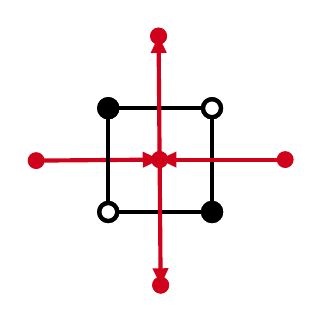
\begin{tikzpicture}[x=0.75pt,y=0.75pt,yscale=-1,xscale=1]
            %uncomment if require: \path (0,410); %set diagram left start at 0, and has height of 410
            
            %Straight Lines [id:da3934001790859082] 
            \draw [line width=1.5]    (261.9,95.25) -- (215.25,95.25) ;
            \draw [shift={(215.25,95.25)}, rotate = 180] [color={rgb, 255:red, 0; green, 0; blue, 0 }  ][fill={rgb, 255:red, 0; green, 0; blue, 0 }  ][line width=1.5]      (0, 0) circle [x radius= 4.36, y radius= 4.36]   ;
            \draw [shift={(265.25,95.25)}, rotate = 180] [color={rgb, 255:red, 0; green, 0; blue, 0 }  ][line width=1.5]      (0, 0) circle [x radius= 4.36, y radius= 4.36]   ;
            %Straight Lines [id:da9659933453892754] 
            \draw [line width=1.5]    (265.25,98.6) -- (265.25,145.25) ;
            \draw [shift={(265.25,145.25)}, rotate = 90] [color={rgb, 255:red, 0; green, 0; blue, 0 }  ][fill={rgb, 255:red, 0; green, 0; blue, 0 }  ][line width=1.5]      (0, 0) circle [x radius= 4.36, y radius= 4.36]   ;
            \draw [shift={(265.25,95.25)}, rotate = 90] [color={rgb, 255:red, 0; green, 0; blue, 0 }  ][line width=1.5]      (0, 0) circle [x radius= 4.36, y radius= 4.36]   ;
            %Straight Lines [id:da9529887421615183] 
            \draw [line width=1.5]    (218.61,145.25) -- (265.25,145.25) ;
            \draw [shift={(265.25,145.25)}, rotate = 0] [color={rgb, 255:red, 0; green, 0; blue, 0 }  ][fill={rgb, 255:red, 0; green, 0; blue, 0 }  ][line width=1.5]      (0, 0) circle [x radius= 4.36, y radius= 4.36]   ;
            \draw [shift={(215.25,145.25)}, rotate = 0] [color={rgb, 255:red, 0; green, 0; blue, 0 }  ][line width=1.5]      (0, 0) circle [x radius= 4.36, y radius= 4.36]   ;
            %Straight Lines [id:da46853719520681536] 
            \draw [color={rgb, 255:red, 208; green, 2; blue, 27 }  ,draw opacity=1 ][line width=1.5]    (236,120.03) -- (180.5,120.5) ;
            \draw [shift={(180.5,120.5)}, rotate = 179.52] [color={rgb, 255:red, 208; green, 2; blue, 27 }  ,draw opacity=1 ][fill={rgb, 255:red, 208; green, 2; blue, 27 }  ,fill opacity=1 ][line width=1.5]      (0, 0) circle [x radius= 3.05, y radius= 3.05]   ;
            \draw [shift={(240,120)}, rotate = 179.52] [fill={rgb, 255:red, 208; green, 2; blue, 27 }  ,fill opacity=1 ][line width=0.08]  [draw opacity=0] (8.13,-3.9) -- (0,0) -- (8.13,3.9) -- cycle    ;
            %Straight Lines [id:da61878858835384] 
            \draw [color={rgb, 255:red, 208; green, 2; blue, 27 }  ,draw opacity=1 ][line width=1.5]    (240.47,176.5) -- (240,120) ;
            \draw [shift={(240,120)}, rotate = 269.53] [color={rgb, 255:red, 208; green, 2; blue, 27 }  ,draw opacity=1 ][fill={rgb, 255:red, 208; green, 2; blue, 27 }  ,fill opacity=1 ][line width=1.5]      (0, 0) circle [x radius= 3.05, y radius= 3.05]   ;
            \draw [shift={(240.5,180.5)}, rotate = 269.53] [fill={rgb, 255:red, 208; green, 2; blue, 27 }  ,fill opacity=1 ][line width=0.08]  [draw opacity=0] (8.13,-3.9) -- (0,0) -- (8.13,3.9) -- cycle    ;
            %Straight Lines [id:da4629638495700332] 
            \draw [color={rgb, 255:red, 208; green, 2; blue, 27 }  ,draw opacity=1 ][line width=1.5]    (244,120) -- (300.5,120) ;
            \draw [shift={(300.5,120)}, rotate = 0] [color={rgb, 255:red, 208; green, 2; blue, 27 }  ,draw opacity=1 ][fill={rgb, 255:red, 208; green, 2; blue, 27 }  ,fill opacity=1 ][line width=1.5]      (0, 0) circle [x radius= 3.05, y radius= 3.05]   ;
            \draw [shift={(240,120)}, rotate = 0] [fill={rgb, 255:red, 208; green, 2; blue, 27 }  ,fill opacity=1 ][line width=0.08]  [draw opacity=0] (8.13,-3.9) -- (0,0) -- (8.13,3.9) -- cycle    ;
            %Straight Lines [id:da8207445621825815] 
            \draw [color={rgb, 255:red, 208; green, 2; blue, 27 }  ,draw opacity=1 ][line width=1.5]    (239.53,64.5) -- (240,120) ;
            \draw [shift={(240,120)}, rotate = 89.52] [color={rgb, 255:red, 208; green, 2; blue, 27 }  ,draw opacity=1 ][fill={rgb, 255:red, 208; green, 2; blue, 27 }  ,fill opacity=1 ][line width=1.5]      (0, 0) circle [x radius= 3.05, y radius= 3.05]   ;
            \draw [shift={(239.5,60.5)}, rotate = 89.52] [fill={rgb, 255:red, 208; green, 2; blue, 27 }  ,fill opacity=1 ][line width=0.08]  [draw opacity=0] (8.13,-3.9) -- (0,0) -- (8.13,3.9) -- cycle    ;
            %Straight Lines [id:da6883475071592661] 
            \draw [line width=1.5]    (215.25,141.9) -- (215.25,95.25) ;
            \draw [shift={(215.25,95.25)}, rotate = 270] [color={rgb, 255:red, 0; green, 0; blue, 0 }  ][fill={rgb, 255:red, 0; green, 0; blue, 0 }  ][line width=1.5]      (0, 0) circle [x radius= 4.36, y radius= 4.36]   ;
            \draw [shift={(215.25,145.25)}, rotate = 270] [color={rgb, 255:red, 0; green, 0; blue, 0 }  ][line width=1.5]      (0, 0) circle [x radius= 4.36, y radius= 4.36]   ;
            %Straight Lines [id:da14590789837946105] 
            \draw [color={rgb, 255:red, 208; green, 2; blue, 27 }  ,draw opacity=1 ][line width=1.5]    (240.5,180.5) ;
            \draw [shift={(240.5,180.5)}, rotate = 0] [color={rgb, 255:red, 208; green, 2; blue, 27 }  ,draw opacity=1 ][fill={rgb, 255:red, 208; green, 2; blue, 27 }  ,fill opacity=1 ][line width=1.5]      (0, 0) circle [x radius= 3.05, y radius= 3.05]   ;
            \draw [shift={(240.5,180.5)}, rotate = 0] [color={rgb, 255:red, 208; green, 2; blue, 27 }  ,draw opacity=1 ][fill={rgb, 255:red, 208; green, 2; blue, 27 }  ,fill opacity=1 ][line width=1.5]      (0, 0) circle [x radius= 3.05, y radius= 3.05]   ;
            %Straight Lines [id:da4482827678046766] 
            \draw [color={rgb, 255:red, 208; green, 2; blue, 27 }  ,draw opacity=1 ][line width=1.5]    (239.5,60.5) ;
            \draw [shift={(239.5,60.5)}, rotate = 0] [color={rgb, 255:red, 208; green, 2; blue, 27 }  ,draw opacity=1 ][fill={rgb, 255:red, 208; green, 2; blue, 27 }  ,fill opacity=1 ][line width=1.5]      (0, 0) circle [x radius= 3.05, y radius= 3.05]   ;
            \draw [shift={(239.5,60.5)}, rotate = 0] [color={rgb, 255:red, 208; green, 2; blue, 27 }  ,draw opacity=1 ][fill={rgb, 255:red, 208; green, 2; blue, 27 }  ,fill opacity=1 ][line width=1.5]      (0, 0) circle [x radius= 3.05, y radius= 3.05]   ;
        \end{tikzpicture}		
    \end{center}
\end{frame}

\begin{frame}{General $n$-face Urban Renewal}
    Let $\Gamma$ be a dimer model with no bivalent nodes. \textbf{General $n$-face urban renewal} of $\Gamma$ at the $n$-face $f$ with nodes $x_1, \ldots, x_n$ consists of the following steps:
    
    \vfill

    \begin{enumerate}
        \item Remove the edges of $f$ from $\Gamma$
        \begin{center}
            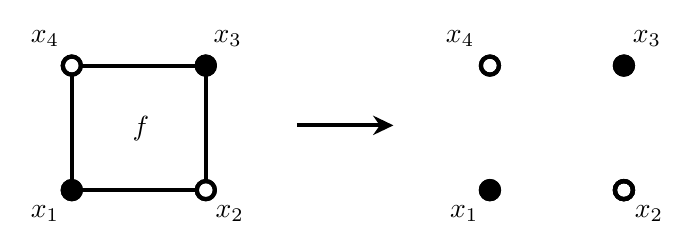
\begin{tikzpicture}[x=0.75pt,y=0.75pt,yscale=-1,xscale=1]
				%uncomment if require: \path (0,410); %set diagram left start at 0, and has height of 410
				
				%Straight Lines [id:da15921640309822205] 
				\draw [line width=1.5]    (142,99.35) -- (142,156) ;
				\draw [shift={(142,156)}, rotate = 90] [color={rgb, 255:red, 0; green, 0; blue, 0 }  ][fill={rgb, 255:red, 0; green, 0; blue, 0 }  ][line width=1.5]      (0, 0) circle [x radius= 4.36, y radius= 4.36]   ;
				\draw [shift={(142,96)}, rotate = 90] [color={rgb, 255:red, 0; green, 0; blue, 0 }  ][line width=1.5]      (0, 0) circle [x radius= 4.36, y radius= 4.36]   ;
				%Straight Lines [id:da5371848830691067] 
				\draw [line width=1.5]    (145.35,96) -- (206.56,96) ;
				\draw [shift={(206.56,96)}, rotate = 0] [color={rgb, 255:red, 0; green, 0; blue, 0 }  ][fill={rgb, 255:red, 0; green, 0; blue, 0 }  ][line width=1.5]      (0, 0) circle [x radius= 4.36, y radius= 4.36]   ;
				\draw [shift={(142,96)}, rotate = 0] [color={rgb, 255:red, 0; green, 0; blue, 0 }  ][line width=1.5]      (0, 0) circle [x radius= 4.36, y radius= 4.36]   ;
				%Straight Lines [id:da6386303020933093] 
				\draw [line width=1.5]    (203.21,156) -- (142,156) ;
				\draw [shift={(142,156)}, rotate = 180] [color={rgb, 255:red, 0; green, 0; blue, 0 }  ][fill={rgb, 255:red, 0; green, 0; blue, 0 }  ][line width=1.5]      (0, 0) circle [x radius= 4.36, y radius= 4.36]   ;
				\draw [shift={(206.56,156)}, rotate = 180] [color={rgb, 255:red, 0; green, 0; blue, 0 }  ][line width=1.5]      (0, 0) circle [x radius= 4.36, y radius= 4.36]   ;
				%Straight Lines [id:da5980285534662942] 
				\draw [line width=1.5]    (206.56,152.64) -- (206.56,96) ;
				\draw [shift={(206.56,96)}, rotate = 270] [color={rgb, 255:red, 0; green, 0; blue, 0 }  ][fill={rgb, 255:red, 0; green, 0; blue, 0 }  ][line width=1.5]      (0, 0) circle [x radius= 4.36, y radius= 4.36]   ;
				\draw [shift={(206.56,156)}, rotate = 270] [color={rgb, 255:red, 0; green, 0; blue, 0 }  ][line width=1.5]      (0, 0) circle [x radius= 4.36, y radius= 4.36]   ;
				%Straight Lines [id:da6265364729689368] 
				\draw [line width=1.5]    (343.44,156) ;
				\draw [shift={(343.44,156)}, rotate = 0] [color={rgb, 255:red, 0; green, 0; blue, 0 }  ][fill={rgb, 255:red, 0; green, 0; blue, 0 }  ][line width=1.5]      (0, 0) circle [x radius= 4.36, y radius= 4.36]   ;
				\draw [shift={(343.44,156)}, rotate = 0] [color={rgb, 255:red, 0; green, 0; blue, 0 }  ][line width=1.5]      (0, 0) circle [x radius= 4.36, y radius= 4.36]   ;
				%Straight Lines [id:da031092445124776824] 
				\draw [line width=1.5]    (408,96) ;
				\draw [shift={(408,96)}, rotate = 0] [color={rgb, 255:red, 0; green, 0; blue, 0 }  ][fill={rgb, 255:red, 0; green, 0; blue, 0 }  ][line width=1.5]      (0, 0) circle [x radius= 4.36, y radius= 4.36]   ;
				\draw [shift={(408,96)}, rotate = 0] [color={rgb, 255:red, 0; green, 0; blue, 0 }  ][line width=1.5]      (0, 0) circle [x radius= 4.36, y radius= 4.36]   ;
				%Straight Lines [id:da7938893362331871] 
				\draw [line width=1.5]    (408,156) ;
				\draw [shift={(408,156)}, rotate = 0] [color={rgb, 255:red, 0; green, 0; blue, 0 }  ][line width=1.5]      (0, 0) circle [x radius= 4.36, y radius= 4.36]   ;
				\draw [shift={(408,156)}, rotate = 0] [color={rgb, 255:red, 0; green, 0; blue, 0 }  ][line width=1.5]      (0, 0) circle [x radius= 4.36, y radius= 4.36]   ;
				%Straight Lines [id:da0874694455685402] 
				\draw [line width=1.5]    (408,156) ;
				\draw [shift={(408,156)}, rotate = 0] [color={rgb, 255:red, 0; green, 0; blue, 0 }  ][line width=1.5]      (0, 0) circle [x radius= 4.36, y radius= 4.36]   ;
				\draw [shift={(408,156)}, rotate = 0] [color={rgb, 255:red, 0; green, 0; blue, 0 }  ][line width=1.5]      (0, 0) circle [x radius= 4.36, y radius= 4.36]   ;
				%Straight Lines [id:da4229049440415611] 
				\draw [line width=1.5]    (250.47,124.8) -- (272.42,124.8) -- (292.95,124.8) ;
				\draw [shift={(296.95,124.8)}, rotate = 180] [fill={rgb, 255:red, 0; green, 0; blue, 0 }  ][line width=0.08]  [draw opacity=0] (9.91,-4.76) -- (0,0) -- (9.91,4.76) -- (6.58,0) -- cycle    ;
				%Straight Lines [id:da8198998926268837] 
				\draw [line width=1.5]    (343.44,96) ;
				\draw [shift={(343.44,96)}, rotate = 0] [color={rgb, 255:red, 0; green, 0; blue, 0 }  ][line width=1.5]      (0, 0) circle [x radius= 4.36, y radius= 4.36]   ;
				\draw [shift={(343.44,96)}, rotate = 0] [color={rgb, 255:red, 0; green, 0; blue, 0 }  ][line width=1.5]      (0, 0) circle [x radius= 4.36, y radius= 4.36]   ;
				
				% Text Node
				\draw (121,162) node [anchor=north west][inner sep=0.75pt]   [align=left] {$\displaystyle x_{1}$};
				% Text Node
				\draw (210,162) node [anchor=north west][inner sep=0.75pt]   [align=left] {$\displaystyle x_{2}$};
				% Text Node
				\draw (209,78) node [anchor=north west][inner sep=0.75pt]   [align=left] {$\displaystyle x_{3}$};
				% Text Node
				\draw (121,78) node [anchor=north west][inner sep=0.75pt]   [align=left] {$\displaystyle x_{4}$};

				% Text Node
				\draw (321,78) node [anchor=north west][inner sep=0.75pt]   [align=left] {$\displaystyle x_{4}$};
				% Text Node
				\draw (411,78) node [anchor=north west][inner sep=0.75pt]   [align=left] {$\displaystyle x_{3}$};
				% Text Node
				\draw (412,162) node [anchor=north west][inner sep=0.75pt]   [align=left] {$\displaystyle x_{2}$};
				% Text Node
				\draw (323,162) node [anchor=north west][inner sep=0.75pt]   [align=left] {$\displaystyle x_{1}$};
				
				% Text Node
				\draw (170,119) node [anchor=north west][inner sep=0.75pt]   [align=left] {$\displaystyle f$};
                % Text Node
				%\draw (370,119) node [anchor=north west][inner sep=0.75pt]   [align=left] {$\displaystyle f$};
			\end{tikzpicture}
        \end{center}
    \end{enumerate}
\end{frame}

\begin{frame}{General $n$-face Urban Renewal (cont.)}
    \begin{enumerate}
        \setcounter{enumi}{1}
        \item Add an $n$-cycle with distinct nodes $y_1, \ldots, y_n$ such that each $y_i$ has opposite color of $x_i$ for each $i$ and add edges $x_iy_i$ for each $i$.
        \begin{center}
            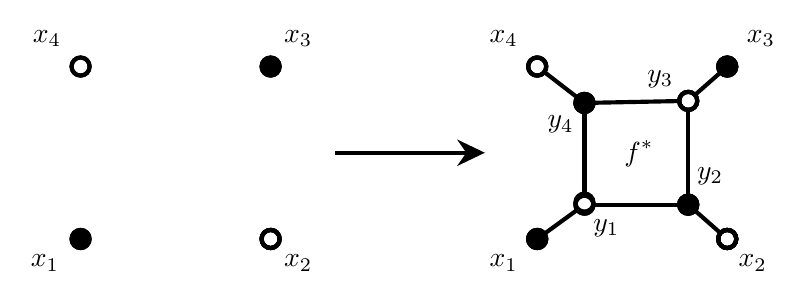
\begin{tikzpicture}[x=0.75pt,y=0.75pt,yscale=-1,xscale=1]
                %uncomment if require: \path (0,410); %set diagram left start at 0, and has height of 410
                
                %Straight Lines [id:da6265364729689368] 
                \draw [line width=1.5]    (129.24,185.54) ;
                \draw [shift={(129.24,185.54)}, rotate = 0] [color={rgb, 255:red, 0; green, 0; blue, 0 }  ][fill={rgb, 255:red, 0; green, 0; blue, 0 }  ][line width=1.5]      (0, 0) circle [x radius= 4.36, y radius= 4.36]   ;
                \draw [shift={(129.24,185.54)}, rotate = 0] [color={rgb, 255:red, 0; green, 0; blue, 0 }  ][line width=1.5]      (0, 0) circle [x radius= 4.36, y radius= 4.36]   ;
                %Straight Lines [id:da031092445124776824] 
                \draw [line width=1.5]    (220.8,102.46) ;
                \draw [shift={(220.8,102.46)}, rotate = 0] [color={rgb, 255:red, 0; green, 0; blue, 0 }  ][fill={rgb, 255:red, 0; green, 0; blue, 0 }  ][line width=1.5]      (0, 0) circle [x radius= 4.36, y radius= 4.36]   ;
                \draw [shift={(220.8,102.46)}, rotate = 0] [color={rgb, 255:red, 0; green, 0; blue, 0 }  ][line width=1.5]      (0, 0) circle [x radius= 4.36, y radius= 4.36]   ;
                %Straight Lines [id:da7938893362331871] 
                \draw [line width=1.5]    (220.8,185.54) ;
                \draw [shift={(220.8,185.54)}, rotate = 0] [color={rgb, 255:red, 0; green, 0; blue, 0 }  ][line width=1.5]      (0, 0) circle [x radius= 4.36, y radius= 4.36]   ;
                \draw [shift={(220.8,185.54)}, rotate = 0] [color={rgb, 255:red, 0; green, 0; blue, 0 }  ][line width=1.5]      (0, 0) circle [x radius= 4.36, y radius= 4.36]   ;
                %Straight Lines [id:da0874694455685402] 
                \draw [line width=1.5]    (220.8,185.54) ;
                \draw [shift={(220.8,185.54)}, rotate = 0] [color={rgb, 255:red, 0; green, 0; blue, 0 }  ][line width=1.5]      (0, 0) circle [x radius= 4.36, y radius= 4.36]   ;
                \draw [shift={(220.8,185.54)}, rotate = 0] [color={rgb, 255:red, 0; green, 0; blue, 0 }  ][line width=1.5]      (0, 0) circle [x radius= 4.36, y radius= 4.36]   ;
                %Straight Lines [id:da8198998926268837] 
                \draw [line width=1.5]    (129.24,102.46) ;
                \draw [shift={(129.24,102.46)}, rotate = 0] [color={rgb, 255:red, 0; green, 0; blue, 0 }  ][line width=1.5]      (0, 0) circle [x radius= 4.36, y radius= 4.36]   ;
                \draw [shift={(129.24,102.46)}, rotate = 0] [color={rgb, 255:red, 0; green, 0; blue, 0 }  ][line width=1.5]      (0, 0) circle [x radius= 4.36, y radius= 4.36]   ;
                %Straight Lines [id:da22684000705984209] 
                \draw [line width=1.5]    (349.24,185.54) ;
                \draw [shift={(349.24,185.54)}, rotate = 0] [color={rgb, 255:red, 0; green, 0; blue, 0 }  ][fill={rgb, 255:red, 0; green, 0; blue, 0 }  ][line width=1.5]      (0, 0) circle [x radius= 4.36, y radius= 4.36]   ;
                \draw [shift={(349.24,185.54)}, rotate = 0] [color={rgb, 255:red, 0; green, 0; blue, 0 }  ][line width=1.5]      (0, 0) circle [x radius= 4.36, y radius= 4.36]   ;
                %Straight Lines [id:da19777547396252992] 
                \draw [line width=1.5]    (440.8,102.46) ;
                \draw [shift={(440.8,102.46)}, rotate = 0] [color={rgb, 255:red, 0; green, 0; blue, 0 }  ][fill={rgb, 255:red, 0; green, 0; blue, 0 }  ][line width=1.5]      (0, 0) circle [x radius= 4.36, y radius= 4.36]   ;
                \draw [shift={(440.8,102.46)}, rotate = 0] [color={rgb, 255:red, 0; green, 0; blue, 0 }  ][line width=1.5]      (0, 0) circle [x radius= 4.36, y radius= 4.36]   ;
                %Straight Lines [id:da36333444172680984] 
                \draw [line width=1.5]    (440.8,185.54) ;
                \draw [shift={(440.8,185.54)}, rotate = 0] [color={rgb, 255:red, 0; green, 0; blue, 0 }  ][line width=1.5]      (0, 0) circle [x radius= 4.36, y radius= 4.36]   ;
                \draw [shift={(440.8,185.54)}, rotate = 0] [color={rgb, 255:red, 0; green, 0; blue, 0 }  ][line width=1.5]      (0, 0) circle [x radius= 4.36, y radius= 4.36]   ;
                %Straight Lines [id:da24554350594858543] 
                \draw [line width=1.5]    (440.8,185.54) ;
                \draw [shift={(440.8,185.54)}, rotate = 0] [color={rgb, 255:red, 0; green, 0; blue, 0 }  ][line width=1.5]      (0, 0) circle [x radius= 4.36, y radius= 4.36]   ;
                \draw [shift={(440.8,185.54)}, rotate = 0] [color={rgb, 255:red, 0; green, 0; blue, 0 }  ][line width=1.5]      (0, 0) circle [x radius= 4.36, y radius= 4.36]   ;
                %Straight Lines [id:da1698713671324199] 
                \draw [line width=1.5]    (349.24,102.46) ;
                \draw [shift={(349.24,102.46)}, rotate = 0] [color={rgb, 255:red, 0; green, 0; blue, 0 }  ][line width=1.5]      (0, 0) circle [x radius= 4.36, y radius= 4.36]   ;
                \draw [shift={(349.24,102.46)}, rotate = 0] [color={rgb, 255:red, 0; green, 0; blue, 0 }  ][line width=1.5]      (0, 0) circle [x radius= 4.36, y radius= 4.36]   ;
                %Straight Lines [id:da08876416120523223] 
                \draw [line width=1.5]    (351.9,104.51) -- (372,120) ;
                \draw [shift={(372,120)}, rotate = 37.61] [color={rgb, 255:red, 0; green, 0; blue, 0 }  ][fill={rgb, 255:red, 0; green, 0; blue, 0 }  ][line width=1.5]      (0, 0) circle [x radius= 4.36, y radius= 4.36]   ;
                \draw [shift={(349.24,102.46)}, rotate = 37.61] [color={rgb, 255:red, 0; green, 0; blue, 0 }  ][line width=1.5]      (0, 0) circle [x radius= 4.36, y radius= 4.36]   ;
                %Straight Lines [id:da8601543366966209] 
                \draw [line width=1.5]    (424.52,116.78) -- (440.8,102.46) ;
                \draw [shift={(440.8,102.46)}, rotate = 318.66] [color={rgb, 255:red, 0; green, 0; blue, 0 }  ][fill={rgb, 255:red, 0; green, 0; blue, 0 }  ][line width=1.5]      (0, 0) circle [x radius= 4.36, y radius= 4.36]   ;
                \draw [shift={(422,119)}, rotate = 318.66] [color={rgb, 255:red, 0; green, 0; blue, 0 }  ][line width=1.5]      (0, 0) circle [x radius= 4.36, y radius= 4.36]   ;
                %Straight Lines [id:da03712904650423743] 
                \draw [line width=1.5]    (438.28,183.32) -- (422,169) ;
                \draw [shift={(422,169)}, rotate = 221.34] [color={rgb, 255:red, 0; green, 0; blue, 0 }  ][fill={rgb, 255:red, 0; green, 0; blue, 0 }  ][line width=1.5]      (0, 0) circle [x radius= 4.36, y radius= 4.36]   ;
                \draw [shift={(440.8,185.54)}, rotate = 221.34] [color={rgb, 255:red, 0; green, 0; blue, 0 }  ][line width=1.5]      (0, 0) circle [x radius= 4.36, y radius= 4.36]   ;
                %Straight Lines [id:da1558026890561699] 
                \draw [line width=1.5]    (369.29,170.97) -- (349.24,185.54) ;
                \draw [shift={(349.24,185.54)}, rotate = 144] [color={rgb, 255:red, 0; green, 0; blue, 0 }  ][fill={rgb, 255:red, 0; green, 0; blue, 0 }  ][line width=1.5]      (0, 0) circle [x radius= 4.36, y radius= 4.36]   ;
                \draw [shift={(372,169)}, rotate = 144] [color={rgb, 255:red, 0; green, 0; blue, 0 }  ][line width=1.5]      (0, 0) circle [x radius= 4.36, y radius= 4.36]   ;
                %Straight Lines [id:da5521811972334515] 
                \draw [line width=1.5]    (372,164.65) -- (372,120) ;
                \draw [shift={(372,120)}, rotate = 270] [color={rgb, 255:red, 0; green, 0; blue, 0 }  ][fill={rgb, 255:red, 0; green, 0; blue, 0 }  ][line width=1.5]      (0, 0) circle [x radius= 4.36, y radius= 4.36]   ;
                \draw [shift={(372,168)}, rotate = 270] [color={rgb, 255:red, 0; green, 0; blue, 0 }  ][line width=1.5]      (0, 0) circle [x radius= 4.36, y radius= 4.36]   ;
                %Straight Lines [id:da5763431474630447] 
                \draw [line width=1.5]    (375.35,169) -- (422,169) ;
                \draw [shift={(422,169)}, rotate = 0] [color={rgb, 255:red, 0; green, 0; blue, 0 }  ][fill={rgb, 255:red, 0; green, 0; blue, 0 }  ][line width=1.5]      (0, 0) circle [x radius= 4.36, y radius= 4.36]   ;
                \draw [shift={(372,169)}, rotate = 0] [color={rgb, 255:red, 0; green, 0; blue, 0 }  ][line width=1.5]      (0, 0) circle [x radius= 4.36, y radius= 4.36]   ;
                %Straight Lines [id:da42043371847712696] 
                \draw [line width=1.5]    (422,122.35) -- (422,169) ;
                \draw [shift={(422,169)}, rotate = 90] [color={rgb, 255:red, 0; green, 0; blue, 0 }  ][fill={rgb, 255:red, 0; green, 0; blue, 0 }  ][line width=1.5]      (0, 0) circle [x radius= 4.36, y radius= 4.36]   ;
                \draw [shift={(422,119)}, rotate = 90] [color={rgb, 255:red, 0; green, 0; blue, 0 }  ][line width=1.5]      (0, 0) circle [x radius= 4.36, y radius= 4.36]   ;
                %Straight Lines [id:da4258870132845348] 
                \draw [line width=1.5]    (418.65,119.07) -- (372,120) ;
                \draw [shift={(372,120)}, rotate = 178.85] [color={rgb, 255:red, 0; green, 0; blue, 0 }  ][fill={rgb, 255:red, 0; green, 0; blue, 0 }  ][line width=1.5]      (0, 0) circle [x radius= 4.36, y radius= 4.36]   ;
                \draw [shift={(422,119)}, rotate = 178.85] [color={rgb, 255:red, 0; green, 0; blue, 0 }  ][line width=1.5]      (0, 0) circle [x radius= 4.36, y radius= 4.36]   ;
                %Straight Lines [id:da7299796873165726] 
                \draw [line width=1.5]    (252,144) -- (320,144) ;
                \draw [shift={(324,144)}, rotate = 180] [fill={rgb, 255:red, 0; green, 0; blue, 0 }  ][line width=0.08]  [draw opacity=0] (13.4,-6.43) -- (0,0) -- (13.4,6.44) -- (8.9,0) -- cycle    ;
                
                % Text Node
                \draw (105,84) node [anchor=north west][inner sep=0.75pt]   [align=left] {$\displaystyle x_{4}$};
                % Text Node
                \draw (226,84) node [anchor=north west][inner sep=0.75pt]   [align=left] {$\displaystyle x_{3}$};
                % Text Node
                \draw (226,192) node [anchor=north west][inner sep=0.75pt]   [align=left] {$\displaystyle x_{2}$};
                % Text Node
                \draw (104.02,192) node [anchor=north west][inner sep=0.75pt]   [align=left] {$\displaystyle x_{1}$};

                % Text Node
                \draw (325,84) node [anchor=north west][inner sep=0.75pt]   [align=left] {$\displaystyle x_{4}$};
                % Text Node
                \draw (449,84) node [anchor=north west][inner sep=0.75pt]   [align=left] {$\displaystyle x_{3}$};
                % Text Node
                \draw (445,192) node [anchor=north west][inner sep=0.75pt]   [align=left] {$\displaystyle x_{2}$};
                % Text Node
                \draw (325,192) node [anchor=north west][inner sep=0.75pt]   [align=left] {$\displaystyle x_{1}$};

                % Text Node
                \draw (375,175) node [anchor=north west][inner sep=0.75pt]   [align=left] {$\displaystyle y_{1}$};
                % Text Node
                \draw (425,150) node [anchor=north west][inner sep=0.75pt]   [align=left] {$\displaystyle y_{2}$};
                % Text Node
                \draw (401,103) node [anchor=north west][inner sep=0.75pt]   [align=left] {$\displaystyle y_{3}$};
                % Text Node
                \draw (353,125) node [anchor=north west][inner sep=0.75pt]   [align=left] {$\displaystyle y_{4}$};
                
                % Text Node
				%\draw (170,137) node [anchor=north west][inner sep=0.75pt]   [align=left] {$\displaystyle f$};
                % Text Node
				\draw (390,137) node [anchor=north west][inner sep=0.75pt]   [align=left] {$\displaystyle f^*$};
            \end{tikzpicture}				
        \end{center}

        \vfill 
        
        \item Apply a join move at each $x_i$ that is bivalent
    \end{enumerate}
\end{frame}

\begin{frame}{Properties of General $n$-face Urban Renewal}
    Can be thought of as a generalization (loosely speaking) of traditional urban renewal ($n = 4$ case) \cite[Section~2.5]{fominIntroductionClusterAlgebras2021a}

    \begin{theorem}
        \justifying
        General $n$-face urban renewal $\rho_f$ at face $f$ has the following properties:
        \begin{enumerate}
            \justifying
            \item It is an involution: $\rho_{f^*}(\rho_f(\Gamma)) \cong \Gamma$
            
            \vspace{0.5cm}
    
            \item Number of faces invariant (i.e. does not annihilate vertices of dimer quiver)
            
            \vspace{0.5cm}
    
            \item Effect on dimer quiver coincides with QP mutation when $n = 4$
        \end{enumerate}
    \end{theorem}
\end{frame}
